\documentclass[a4paper, 11pt, oneside, polutonikogreek, german]{article}
\usepackage{gfsbaskerville}
% Load encoding definitions (after font package)
\usepackage[LGR,T1]{fontenc}

\usepackage{textalpha}
\usepackage{bbding}
\usepackage{listings}
\lstset{basicstyle=\ttfamily}
\usepackage{wasysym}
\usepackage{cjhebrew}
\usepackage{semtrans}
\makeatletter
\renewcommand*\U[1]{\oalign{#1\crcr\hidewidth\ltx@sh@ft{-3ex}%
   \vbox to .2ex{\hbox{\u{}}\vss}\hidewidth}}
\makeatother

\usepackage[dvipsnames]{xcolor}
\usepackage{eso-pic,graphicx}
\usepackage[top=68mm, bottom=97mm, outer=50mm, inner=50mm]{geometry}
\setlength{\columnsep}{90pt}
\usepackage{etoolbox}    % for \patchcmd
\usepackage{sectsty}
\usepackage{tocloft}

\allsectionsfont{\bfseries}
\sectionfont{\bfseries}
\subsectionfont{\bfseries}
\subsubsectionfont{\bfseries}

% change color of text, example replace all \color{Goldenrod} with \color{lightgray}
\definecolor{myColor}{RGB}{0, 86, 63}

\makeatletter % change only the display of \thepage, but not \thepage itself:
\patchcmd{\ps@plain}{\thepage}{\bfseries\color{Black}{\thepage}}{}{}
\makeatother

\color{Black}

% Babel package:
\usepackage[german]{babel}

% With XeTeX$\$LuaTeX, load fontspec after babel to use Unicode
% fonts for Latin script and LGR for Greek:
\ifdefined\luatexversion \usepackage{fontspec}\fi
\ifdefined\XeTeXrevision \usepackage{fontspec}\fi

% "`Lipsiakos"' italic font `cbleipzig`:
\newcommand*{\lishape}{\fontencoding{LGR}\fontfamily{cmr}%
		 \fontshape{li}\selectfont}
\DeclareTextFontCommand{\textli}{\lishape}
\usepackage{booktabs}
\setlength{\emergencystretch}{15pt}
\usepackage{fancyhdr}
\usepackage{microtype}
\usepackage{graphicx}
\usepackage{float}
\usepackage{caption}

\begin{document}
\bfseries
\AddToShipoutPictureBG{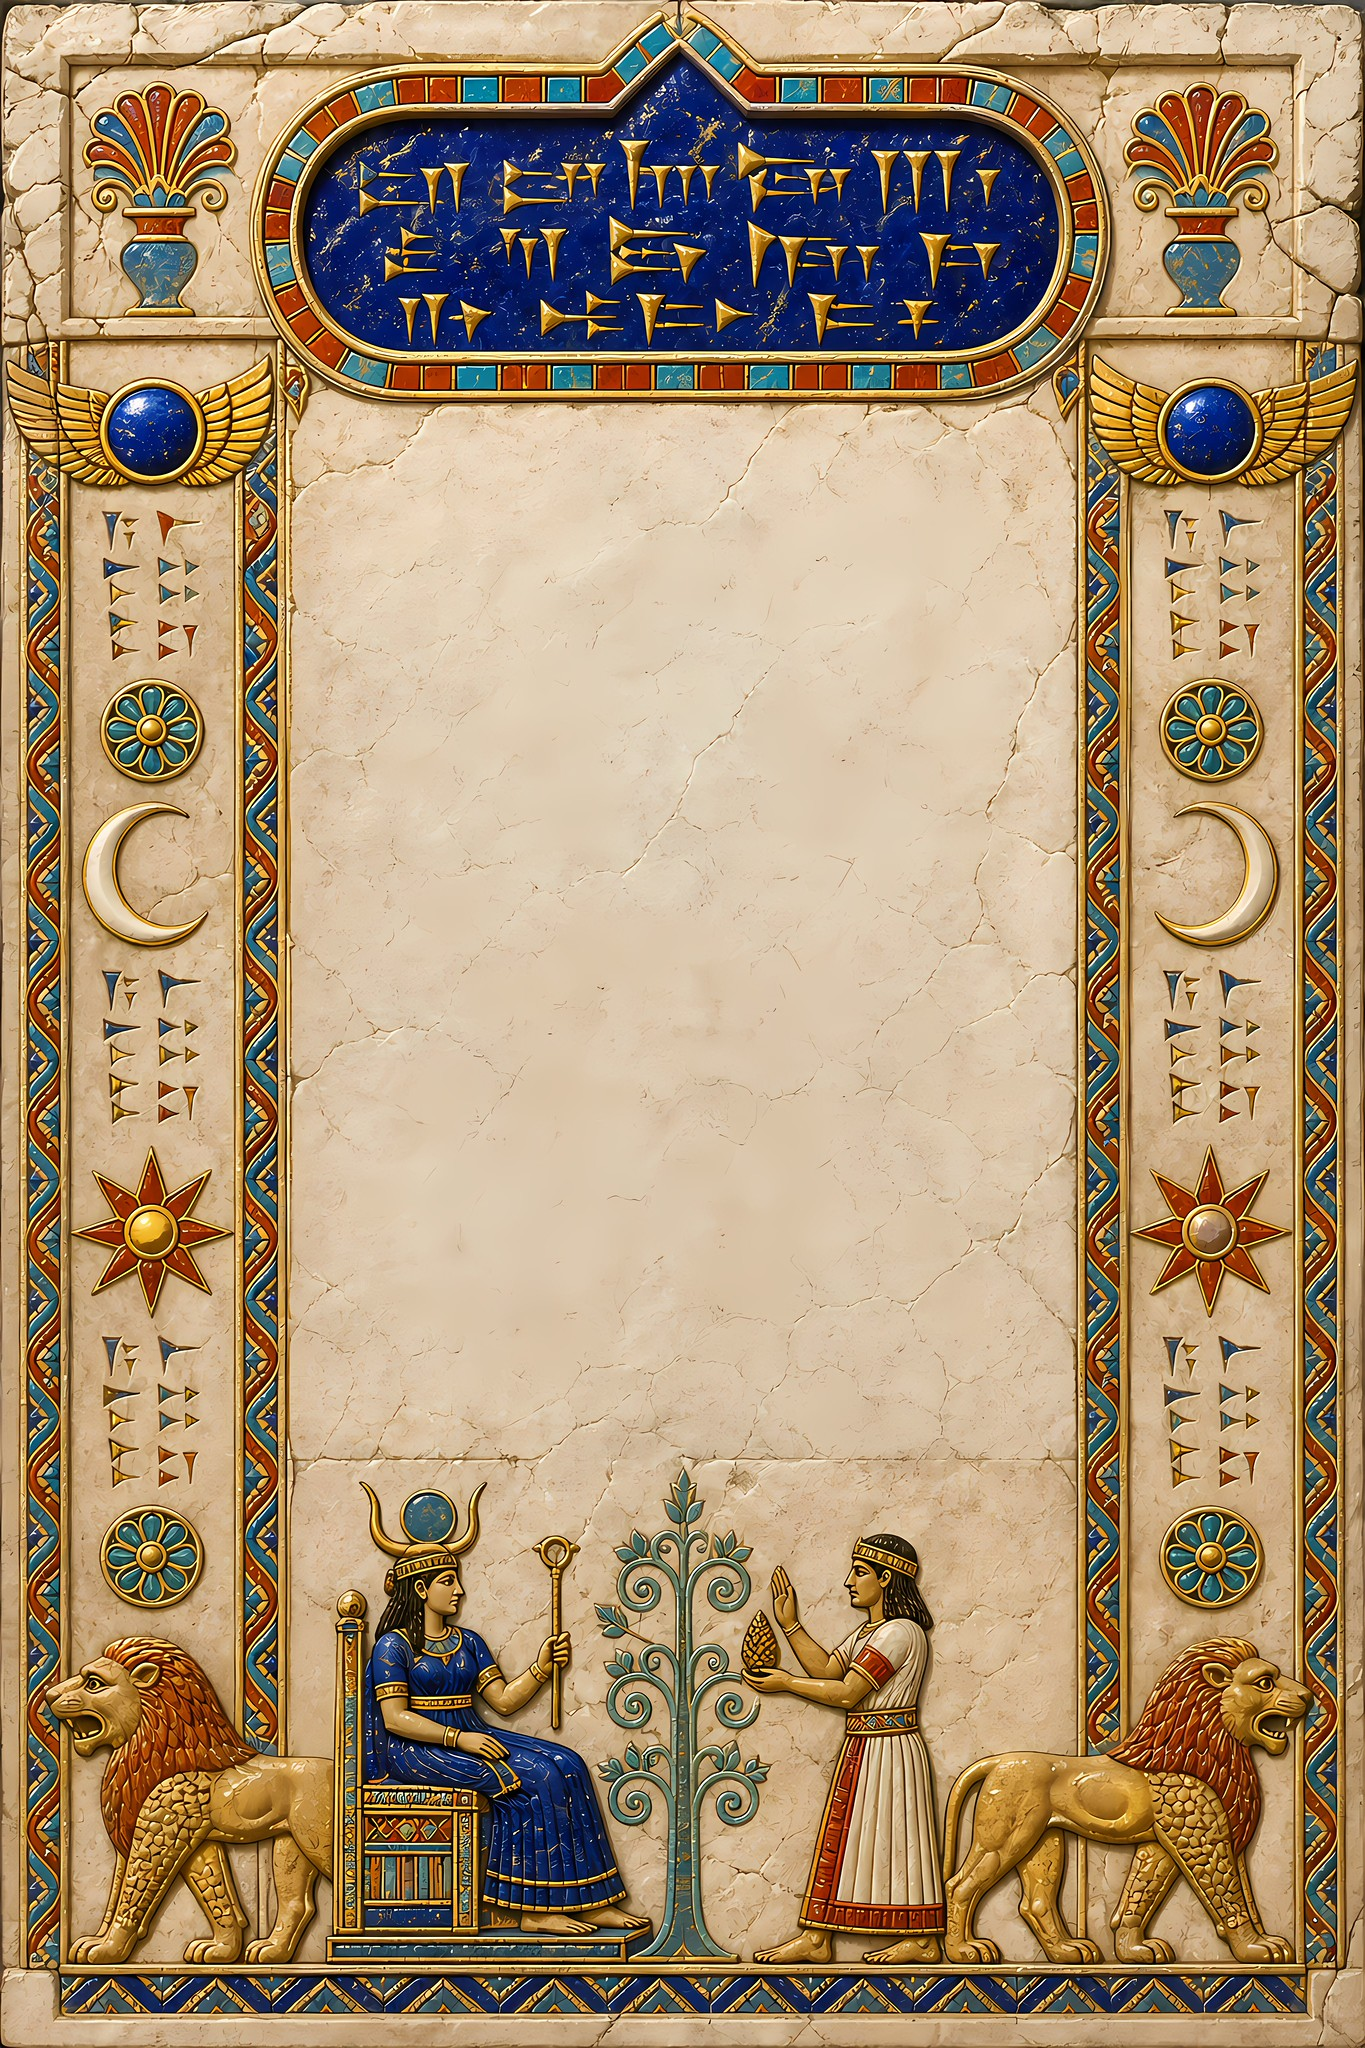
\includegraphics[width=\paperwidth,height=\paperheight]{assyrianstele2.jpg}}
\renewcommand\thefootnote{\scriptsize\bfseries{\arabic{footnote}}}
\let\oldfootnote\footnote
    \renewcommand{\footnote}[1]{\oldfootnote{\bfseries\scriptsize#1}}
\fancypagestyle{plain}{%
\fancyhf{} % clear all header and footer fields
\fancyfoot[C]{\bfseries\scriptsize\thepage} % except the center
\renewcommand{\headrulewidth}{0pt}
\renewcommand{\footrulewidth}{0pt}
}
\pagestyle{plain}
\begin{titlepage}
    \centering                     % Center everything on the page

    % -------------------------------------------------
    % Title rules
    % -------------------------------------------------
    \rule{\textwidth}{1.6pt}\\[-\baselineskip]\vskip2pt
    \rule{\textwidth}{0.4pt}\\[1\baselineskip]

    % -------------------------------------------------
    % Title
    % -------------------------------------------------
    {\scshape\Huge Die historische Semiramis\\ und ihre Zeit}\\[1\baselineskip]

    % -------------------------------------------------
    % Bottom title rules
    % -------------------------------------------------
    \rule{\textwidth}{0.4pt}\\[-\baselineskip]\vskip3.2pt
    \rule{\textwidth}{1.6pt}\\[1\baselineskip]

    % -------------------------------------------------
    % Autho
    % -------------------------------------------------
    
    {\scshape Von \\\Large C. F. Lehmann-Haupt}

    % -------------------------------------------------
    % Date / defense statement / author line
    % -------------------------------------------------

    {\scshape \small Vortrag gehalten in der Deutschen Orient-Gesellschaft zu Berlin am 6. Februar 1910\\ Mit 50 Abbildungen}


    % -------------------------------------------------
    % Place / publisher info (pushed to bottom)
    % -------------------------------------------------

    \vfill

    {\scshape\small Verlag von J. C. B. Mohr (Paul Siebeck)}

    {\scshape Tübingen 1910}

    % -------------------------------------------------
    % Edition / license line
    % -------------------------------------------------
    {\scshape Solar Anamnesis Edition}\\[0.2\baselineskip]
    {\scshape\small CC0 1.0 Universell}
\end{titlepage}
\setlength{\parskip}{1mm plus1mm minus1mm}
\clearpage
\begin{figure}[H]
\centering
\includegraphics[width=\textwidth,height=\textheight,keepaspectratio]{figures-trans/Figure-001.png}
\caption*{\bfseries\small \textsc{Alte Tigrisbrücke bei Djezîreh. (Zeichnung von Eugen Hanetzog.)}}
\end{figure}
\paragraph{}
Trotz der sagenhaften Umhüllung, in der die Nachrichten über Ninos und Semiramis uns bei Ktesias entgegentreten, konnte man ehedem glauben, dass wirklich am Anfang der Geschichte des gesamten Zweistromlandes als Begründerin Ninives oder gar Babylons eine Herrscherin des Namens Semiramis gestanden hätte. Diese Zeiten sind endgültig vorbei. Die Entzifferung der Keilschrift durch Georg Friedrich Grotefend und die Erschließung der inschriftlichen Schätze des Zweistromlandes lehrten uns die Anfänge der Geschichte Babyloniens und des von ihm erst nachträglich sich ablösenden Assyrien kennen: für eine Reichsgründerin Semiramis fand sich dort nirgends eine Spur noch Raum. So hätte man denken können, dass, was Ktesias, der als Leibarzt des persischen Großkönigs Artaxerxes 2. um 400 v. Chr. in Susa lebte, über die Semiramis berichtete, Sage, nichts als Sage sei, die er der iranischen Volksüberlieferung --- den Gesängen und Mären der Meder und Perser --- abgelauscht habe.

Da das Perserreich den ganzen vorderen Orient umfasste, so ließ sich damit auch die Tatsache vereinigen, dass der Geburtsort der Semiramis ins westliche Syrien verlegt wurde: dort sei ihr, die einst --- von den Tauben,\footnote{Die Rolle die die Taube in der Semiramis-Sage spielt, beruht wohl teils darauf, dass die Taube der Istar heilig ist (s. dazu H. Zimmern, Die Keilinschriften und das alte Testament, 3. Aufl., S. 429, 431 Anm. 5, 440) teils auf einem leichten Anklang des Namens der Semiramis an ein semitisches Wort für „Taube“ (bab.-assyr. summatu)} den heiligen Vögeln der Astarte wie der Aphrodite, genährt --- unter der Obhut eines Hirten aufgewachsen war und die dann als Gemahlin eines andern vom Könige Ninos zum Weibe begehrt wurde --- göttliche Verehrung zuteilgeworden.

Aber auch der Gedanke, dass es sich um eine reine Sagengestalt, um eine historisch in keiner Weise greifbare Persönlichkeit handle, musste, ehe er noch Wurzel fassen konnte, aufgegeben werden.

Die ersten epochemachenden englischen Entdeckungen im Zweistromlande erfolgten in den heute Nimrud genannten Ruinen der altassyrischen Residenzstadt Kalach, die --- etwas südlich von Ninive gelegen --- auch im Alten Testamente genannt wird. Schon ein Jahrzehnt nach dem Beginn der Ausgrabungen wurde dort eine auf mehreren Statuen des Gottes Nebo (Abb. S. 3) gleichlautend wiederholte Inschrift gefunden --- dem Gotte geweiht vom Statthalter von Kalach für das Leben Adadniraris (um 800 v. Chr.) und seiner „Palastfrau,“ die den mit Semiramis so gut wie völlig identischen Namen Schammuramat führte.\footnote{Die Angaben über die Zahl der Nebo-Statuen schwanken. Anfänglich (1851) wurden zwei beschriebene Statuen gefunden (W. K. Loftus, Travels and researches in Chaldaea and Susiana p. 271 ff.). Sir Henry Rawlinson, The cuneiform inscriptions of Western Asia 1. pl. 35 No. 2, erwähnt im Ganzen fünf lebensgroße beschriebene und zwei kolossale unbeschriebene Statuen, von den ersteren seien zwei im Britischen Museum. George Rawlinson dagegen (The five great monarchies of the East, vol. 2 p. 119 ff.) weiß von vier beschriebenen und vier inschriftlosen kolossalen Statuen zu berichten, die sein Bruder Henry gefunden habe.}

Sie war also --- so musste man zunächst annehmen, die Gattin Adadniraris, wie denn in einem Briefe, den Goethe im „Westöstlichen Divan,“ wenn auch schwerlich in ganz richtiger Übersetzung, wiedergibt, der Schah von Persien zum Kaiser von Russland von der Zarin als von der „Frau des Palastes“ spricht. Schon die Erwähnung einer Frau in einer offiziellen Urkunde war an sich etwas höchst Außergewöhnliches. Zudem bezeichnet sie der Statthalter als seine Herrin, genau wie den König als seinen Herrn. So ergab sich, dass tatsächlich in Assyrien eine Herrscherin Semiramis gelebt hatte, von ungewöhnlicher Bedeutung und wohl geeignet zum Mittelpunkt eines Legendenkreises, dessen Entstehung im einzelnen man nachzugehen versuchen konnte. ---

\begin{figure}[H]
\centering
\includegraphics[height=0.85\textheight,keepaspectratio]{figures-trans/Figure-002.png}
\caption*{\bfseries\small \textsc{Nebo-Statue aus Kalach-Nimrud.}}
\end{figure}
\paragraph{}
Dass sie die Gemahlin Adadniraris war, erschien zwar, wie bemerkt, als das Nächstliegende, aber nicht als das einzig Denkbare. Über ihre Stellung innerhalb des assyrischen Königshauses hat erst die allerjüngste Zeit Klarheit geschaffen durch einen bei den Ausgrabungen unserer Deutschen Orient-Gesellschaft in Assur gewonnenen Fund: einen Denkstein, der wohl als der wichtigste unter einer ganzen Gruppe höchst eigenartiger Monumente zu bezeichnen ist.

Unweit einer der Befestigungsmauern von Assur sind nach und nach zwei einander parallele Reihen von Stelen gefunden worden, eine nördlichere und eine südlichere. Nur wenige stehen noch aufrecht (vgl. Abb. S. 5). Manche von ihnen sind mit der Vorderseite nach unten zu Boden gestürzt, von den Sockeln herunter, in die ihr zapfenartig auslaufendes Ende eingelassen war. Die Stelen der einen Reihe (Abb. S. 6) tragen Inschriften von assyrischen Herrschern, die andre weist auf ihren Steinsäulen nur die Namen von Statthaltern und Großwürdenträgern auf. Meist zeigen sie die Form viereckiger Steinpfeilern, die ihrer Anlage nach niemals ein Bildwerk getragen haben können. Das zu Beginn ihrer Inschriften stets erscheinende assyrische Wort, das man bisher als Bildsäule auffasste, wird daher auch die Bedeutung Denksäule gehabt haben. Diese Inschrift ist jedesmal im oberen Teil der Vorderseite in einer vertieften Nische von der Form eines Amuletts angebracht. Abweichender Form sind namentlich nur eine sehr verstümmelte, 4 m hohe Königsstatue und ein achtseitiger Basaltpfeiler. Eine in ihrer Anlage ganz ähnliche, aber inschriftlose Stelenreihe ist, wie beiläufig bemerkt sei, bei den englischen Ausgrabungen in der palästinensischen Stadt Gezer gefunden worden. Freilich handelt es sich dort schwerlich um Denksäulen für Herrscher und Statthalter, während andrerseits der Gedanke, es seien die zwölf Stämme Israels mit je einer Stele zum Zwecke des Kultus vertreten, noch weiterer Prüfung bedarf.

\begin{figure}[H]
\centering
\includegraphics[width=\textwidth,height=\textheight,keepaspectratio]{figures-trans/Figure-003.png}
\caption*{\bfseries\small \textsc{Assur: Zwei Königsstelen.}}
\end{figure}

\begin{figure}[H]
\centering
\includegraphics[width=\textwidth,height=\textheight,keepaspectratio]{figures-trans/Figure-004.png}
\caption*{\bfseries\small \textsc{Assur: Die Reihe der Königsstelen aus Westen.}}
\end{figure}
\paragraph{}
%כלּה
Eine der Stelen der monumentalen Königsliste von Assur trägt nun die folgende Inschrift:\footnote{Zeile 6 der Semiramis-Inschrift von Assur beginnt nach den von dorther eingetroffenen Berichten mit den Zeichen KID. LAT. --- Die Annahme liegt sehr nahe, dass für KID das ihm sehr ähnliche Zeichen KAL dasteht und dann zu lesen ist kal-lat. Damit würde Semiramis (in assyrischer Aussprache: Schammuramat, in babylonischer: Sammuramat) bezeichnet als die Schwiegertochter Salmanassars 3. (Kallâtu bezeichnet zwar ursprünglich „Braut, junge Frau.“ Aber auch im Hebräischen findet sich für \<kl*h> kallâh der gleiche Bedeutungsübergang, der auch bei dem griechischen Worte νύμφη, besonders im Neuen Testament, nachweisbar ist). Freilich griffe dann die Genealogie die im Übrigen in dieser Inschrift von oben nach unten fortschreitet, zurück. Erwiese sich dagegen bei Prüfung des Originals, dass wirklich KID. LAT dasteht, so müsste, wie im Text bemerkt, Semiramis dadurch als Großmutter oder Vormundin Salmanassars 4. charakterisiert sein.}
\begin{quotation}\small
„Säule der Schammuramat,

Der Frau des Palastes Samsi-Adads,

Des Königs der Welt, Königs von Assyrien;

Der Mutter Adadniraris,

Des Königs der Welt, Königs von Assyrien;

Der ... des Sulmanuasaridu, Königs

Der vier Weltgegenden.“
\end{quotation}
\begin{figure}[H]
\centering
\includegraphics[width=0.85\textwidth,keepaspectratio]{figures-trans/Figure-005.png}
\caption*{\bfseries\small \textsc{Inschrift der Semiramis-Stele von Assur.}}
\end{figure}
\paragraph{}
Semiramis war also die Mutter Adadniraris 4., als dessen Palastfrau sie in der Inschrift auf der Nebostatue genannt wurde. Sie ist die einzige Frau, die in dieser Reihe von Denksteinen mit einer solchen Stele vertreten ist. Auch hat man sich nicht begnügt, von ihr etwa zu sprechen als von der Gemahlin Samsi-Adads, des Vaters Adadniraris, sondern das Verhältnis der königlichen Frau zu drei Assyrerkönigen wird besonders hervorgehoben. Den an dritter Stelle erscheinenden Namen Salmanassar trägt sowohl der Vater ihres Gemahls, Salmanassar 3., wie der Nachfolger des Sohnes, Salmanassar 4. Die diesem Namen vorausgehenden Keilschriftgruppen sind nicht völlig klar. Die Königin wird durch sie entweder als Großmutter oder Vormundin des jüngeren Salmannassar oder aber, und wohl wahrscheinlicher, als Schwiegertochter des älteren genannt sein.

Wie dem immer sei: die zeitlichen Grenzen für unsere Betrachtung sind durch die Regierungen dieser beiden gleichnamigen Herrscher jedenfalls gegeben.

Auf unsrer Stele wird Semiramis als Palastfrau Samsi-Adads, ihres Gemahls, bezeichnet. Dieselben Titel erhält auf einer ebenfalls in der Nähe des Stelenplatzes neuerdings gefundenen Skulptur auch die Gemahlin Assurbanabals, die auf dem wohlbekannten Relief mit ihrem Gemahl gemeinsam in der Weinlaube dargestellt ist. Wenn dieser Titel, wie die länger bekannte Inschrift auf der Nebostatue uns zeigt, der Semiramis auch unter der Regierung ihres Sohnes verblieben ist, so spricht auch das für das Vorhandensein und die Fortdauer eines außergewöhnlichen, weit über das Frauengemach hinausreichenden Einflusses auf die eigentlichen Regierungsmaßnahmen, der ihrem Sohne schwerlich immer willkommen gewesen sein wird.

Und merkwürdigerweise hat sich auch in der Semiramis-Sage eine Hindeutung auf dieses Verhältnis erhalten, die wir erst jetzt, da wir wissen, dass Schammuramat die Mutter Adadniraris gewesen, als einen historischen Zug voll zu würdigen imstande sind. Ninyas, ihr Sohn --- so hören wir durch Ktesias --- habe durch einen Eunuchen einen Anschlag auf das Leben der Semiramis versucht; sie aber habe ihrem Sohne nach dessen Entdeckung nicht nur nichts Übles zugefügt, sondern ihm die Herrschaft übergeben und die Statthalter angewiesen, ihm zu gehorchen. Sie selbst aber habe sich das Leben genommen, als sei sie in Erfüllung eines Orakelspruchs zu den Göttern entrückt. Andre behaupteten, sie sei in eine Taube verwandelt worden.\footnote{Der Sohn (811-783) der Semiramis als Adadnirari 4 (nicht, wie bisher als „3“) zu bezeichnen s. Mitteilungen der Deutschen Orient-Gesellschaft No. 2 35 u. S. 32 S. 19 und Klio 6. (1906), S. 534 f. Ihr Schwiegervater (860-26) als Salmanassar 3 (nicht „2“) nach F. Delitzsch, Mitt. d. D. Or.-G. No. 42, S. 35 Anm.}

\begin{figure}[H]
\centering
\includegraphics[height=0.85\textheight,keepaspectratio]{figures-trans/Figure-006.png}
\caption*{\bfseries\small \textsc{Salmanassar 3., der Schwiegervater der Semiramis.}}
\end{figure}
\paragraph{}
Dass kriegerischer Sinn und bedeutende Eroberungszüge der sagenhaften Vertreterin des kriegerischen Assyrerreiches zugeschrieben wurden, war an sich selbstverständlich. Nun aber trifft weiter zu, dass die Zeit, in der die geschichtliche Semiramis lebte, an kriegerischen Unternehmungen besonders reich war. Salmanassar 3. (860-826), ihr Schwiegervater, hat seine Waffen im Süden nach Babylonien, im Westen gegen Damaskus, Hamat und deren Verbündete, nicht minder auch nach Osten und Norden getragen, wie uns denn der bekannte Obelisk Salmanassars aus Kalach-Nimrud die Erfolge, die der Herrscher in allen Himmelsrichtungen errungen hatte, in den Tributen und Geschenken der unterworfenen und bekämpften Völker --- darunter dem des Jehu von Israel --- vor Augen führt. Sein Sohn aber, der Gemahl, und sein Enkel, der Sohn der Semiramis, haben es ihm nachgetan.

Zwei Völkerschaften treten in dem sagenhaften Berichte bei Ktesias besonders hervor, im Osten die Meder, im Norden die damaligen Bewohner des nachmals als Armenien bezeichneten Gebietes.

Und darin klingen nicht minder geschichtliche Vorgänge aus den Zeiten der Semiramis nach, Vorgänge, die zudem den Schlüssel zur Entstehung der Sage in sich bergen.

Mit den Medern, dem ersten arischen Volk, das von Norden her im Osttigrislande erschien, ist zuerst der Schwiegervater der Schammuramat in feindliche Berührung gekommen; ebenso hat ihr Gemahl einen, ihr Sohn dagegen als König acht Feldzüge gegen sie richten müssen.

Die Kämpfe mit den Bewohnern des späteren Armeniens wiederum sind ein der Sage von Ninos und Semiramis besonders fest und zäh anhaftender Zug; er begegnet uns noch in einem neuerdings auf einem Papyrus in Ägypten gefundenen Ninos-Roman wieder,\footnote{Der Ninos-Roman herausgegeben und behandelt von U. Wilcken, Hermes 28 (1893), S. 161 ff.} der im übrigen die Personen und Motive der Sage gründlich umgestaltet. Namentlich ist aus Ninos ein tugend- und empfindsamer Jüngling, aus seiner Erwählten, die schlechtweg als „die Maid“ ohne Namensnennung bezeichnet wird, das Musterbild einer sittigen Jungfrau geworden. Trotzdem aber lässt der Dichter, der offenbar gar keine Vorstellung von den ungeheuren Schwierigkeiten hat, die ein Kriegszug von Assyrien aus gegen das armenische Bergland mit sich brachte, den Ninos mit seinen 150 Elefanten gegen Armenien ziehen. Ktesias aber lässt nicht nur --- eine im Grunde gewiss richtige Beobachtung --- die Semiramis das Steinmaterial zu den assyrischen Stelen den armenischen Gebirgen entnehmen, sondern er berichtet auch, dass Ninos, ehe er gegen die Meder zog, die Bewohner Armeniens und ihren König besiegt, dann aber diesem die Herrschaft großmütig belassen habe. Darin spiegelt sich in eigentümlicher, aber deutlicher Weise die geschichtliche Wahrheit wieder, dass von allen Völkern und Reichen Vorderasiens in der Tat nur ein zu den Zeiten der Semiramis im armenischen Berglande blühendes Reich den Assyrern nachhaltig widerstanden und ihnen gegenüber seine Selbständigkeit bis zu Ende aufrechterhalten hat.\footnote{Steintransport aus Armenien durch Semiramis Diodor 2, 11, 4. --- Ninos gegen Armenien: Diodor 2, 1, 8 u. 9.}

Das Quellgebiet der Ströme, die die Lebensader ihres Landes bildeten, musste Babyloniern und Assyrern von jeher bedeutsam und verlockend erscheinen, schon weil die wichtigste Erscheinung im Leben der Ströme und des Landes, das jährliche gewaltige Anschwellen der Wassermassen, durch die Schneeschmelze in den armenischen Gebirgen --- wie das auch Herodot betont --- veranlasst wurde. Die uralte Verehrung der Quellen und die Schwierigkeit des Vordringens zu ihnen gaben einen weiteren Anreiz zu kriegerischen Entdeckungszügen, die, schon bald nachdem Assyrien um die Mitte des zweiten vorchristlichen Jahrtausends sich von Babylonien unabhängig gemacht hatte, zum Teil mit bedeutendem Erfolge ins Werk gesetzt wurden.

Gerade zu den Zeiten der Semiramis aber vollzog sich im Quellgebiet der beiden Ströme eine bedeutsame Veränderung Ein neues, wahrscheinlich von Westen eingewandertes, freiheitliebendes und kampfesfrohes Volk, die Urartäer, unter einem kraftvollen und zielbewussten Herrscherhause, vereinigte die Naïri-Völker, die bisher zerstreuten Stämme des armenischen Berglandes, zu einem mächtigen Reiche Urartu, dessen Name in einer etwas abweichenden Form uns allen von Jugend an wohlvertraut ist: blieb doch auf einem Berge des Landes Ararat die Arche Noä haften.

Die Urartäer, die als Hauptgott den Chaldis verehrten und deshalb auch als Chalder bezeichnet werden, haben von den Assyrern, deren Lehrmeister sie in vieler Hinsicht geworden sind, die Keilschrift fast unverändert übernommen und für ihre, freilich mit dem Assyrischen nicht verwandte Sprache verwendet. So kommt es, dass den assyrischen Berichten aus den Zeiten der Semiramis gleichzeitige, urartäische Nachrichten, sie kontrollierend, gegenüberstehen. Das ist von hoher Wichtigkeit; denn eine einigermaßen objektive Würdigung fremdländischer Verhältnisse ist mit dem Charakter der assyrischen Königsinschriften ebenso unverträglich wie mit dem der ägyptischen und römischen Berichte. Jeder Widerstand gegen das Vordringen Assurs wird als Rebellion bezeichnet. Angeblich sind die Assyrer immer erfolgreiche Sieger. Wie viele Niederlagen und Misserfolge dabei vertuscht werden, kann man aus ihren Berichten allein nur gelegentlich ahnen.

So sind wir über die urartäisch-assyrischen Beziehungen zur Zeit der Semiramis besonders ausgiebig unterrichtet. Da es nun an gleichzeitigen medischen Nachrichten, auf die wir für unsre Betrachtung noch größeren Wert zu legen hätten, völlig mangelt, so bleiben wir, wenn wir uns die kampferfüllte Zeit der Semiramis möglichst lebendig vor Augen führen wollen, darauf angewiesen, die kriegerischen Verwicklungen zwischen den Assyrern und den Urartäern, den vorarmenischen Bewohnern des Quellgebiets der beiden Ströme, in den Mittelpunkt unsrer Betrachtung zu rücken.

Es kommt hinzu, dass eine Dankespflicht gegen einen deutschen Pionier der Keilschriftforschung, der als ein Opfer wissenschaftlichen Forschungsdranges und Wagemutes sein Leben gelassen hat, die Blicke in diese Richtung zwingt.

Lange ehe die französischen und englischen Ausgrabungen im Zweistromlande begonnen wurden, hat ein junger hessischer Gelehrter, Professor Eduard Schulz, auf Anregung Karl Ritters Armenien bereist (1828), und dort zahlreiche Keilschriften entdeckt und kopiert, welche in der Umgebung von Van, zumeist in Felsen gehauen, sich vorfanden und der Semiramis zugeschrieben wurden.

Und noch ein andres geschichtliches Interesse wohnt diesem einstigen Schauplatze der assyrischurartäischen Kriegszüge inne. Hier war es, wo unser Moltke, als Offizier in türkischen Diensten, in den Kurdenkriegen die ersten Erfahrungen in der praktischen Strategie sammelte, als deren Meister er sich --- Deutschland zum Heile --- ein Menschenalter später erweisen sollte. Er war es auch, der, als er im Jahre 1840 von der türkischen Provinzialhauptstadt Charput zum Euphrat gezogen kam, dort an einem Felsen die westlichste und eine der allerwichtigstenvorarmenischen Keilinschriften entdeckte, in der Nähe einer nach urartäischer Weise in den lebendigen Fels gehauenen Festungsanlage mit einem künstlichen Durchblick nach dem benachbarten wichtigen Euphrat-Übergang. (Abb. S. 15).

Ich selbst aber bin in der glücklichen Lage, die Schauplätze dieser Züge und Kämpfe und mancher Altertümer, die sich aus dieser Urzeit erhalten haben, aus eigener Anschauung zu schildern und abzubilden, wie ich sie auf einer mit Förderung und Unterstützung Sr. Majestät des Kaisers 1898/99 unternommenen Forschungsreise vorgefunden und aufgenommen habe.

\begin{figure}[H]
\centering
\includegraphics[height=0.9\textheight,keepaspectratio]{figures-trans/Figure-007.png}
\caption*{\bfseries\small \textsc{Künstlicher Durchblick an einer chaldischen Felsenfeste. (Zeichnung von Franz Frohse).}}
\end{figure}
\paragraph{}
Von meinen Routen kommt, entsprechend den beiden Hauptkriegsschauplätzen, für uns besonders das Stück zwischen Niniveh und dem Gebiet der beiden Tigrisquellströme, --- des Ost-Tigris oder Bohtan-su und des bei Argana zwischen Charput und Dijarbekir entspringenden West-Tigris --- und ferner das Gelände zwischen dem Van-See und dem Urmia-See in Betracht. --- Folgen wir zunächst Salmanassar 3., dem Schwiegervater der Semiramis, auf seinen Kriegszügen gegen die Urartäer.

\begin{figure}[H]
\centering
\includegraphics[width=\textwidth,height=\textheight,keepaspectratio]{figures-trans/Figure-008.png}
\caption*{\bfseries\small \textsc{Blick in das Tal des Bohtau-su (Kentrites), südlich von Söört. (Zeichnung von Franz Frohse).}}
\end{figure}
\paragraph{}
Bei Djezîreh, in dessen Nachbarschaft der Tigris überschritten wird, blicken wir nordwärts zum Djebel Djudi, der --- zu den südlichen Randgebirgen des Landes Ararat gehörig --- vielfach als der Gebirgsstock gilt, an dem das Schiff des Xisuthros, des babylonischen Noah, durch Cyklone und Springfluten aus dem persischen Golfe nach Norden getrieben, einstmals haften geblieben ist. Eine großartige Brückenruine aus mongolischer oder persischer Zeit gibt heute einen eindrucksvollen Rahmen für das herrliche Landschaftsbild ab. (Abb. S. 1).

Den Ost-Tigris südlich von Söört zu überschreiten, erweist sich wegen der Steilheit der Uferberge zu beiden Seiten, zwischen denen der Strom in tiefer Schlucht dahinfließt, als unmöglich. Erst westlich von Söört, kurz oberhalb der Vereinigung des Bohtan-su mit dem West-Tigris, kann das urartäische Ufer erreicht werden, in der Nachbarschaft der Furt, die im Jahre 404 die zehntausend Griechen auf ihrem Rückzuge benutzt haben. Und an dem Zusammenfluss der beiden Tigrisarme wird Rast und Umschau gehalten.

Schon Salmanassars 3. Vater erwähnt die Stadt und Feste Tilla unter dem Namen, den sie noch heute führt.

\begin{figure}[H]
\centering
\includegraphics[width=\textwidth,height=\textheight,keepaspectratio]{figures-trans/Figure-009.png}
\caption*{\bfseries\small \textsc{Zusammenfluss des Ost-Tigris (Bohtan-su) mit dem West-Tigris bei Till. (Zeichnung von Lucy du Bois-Reymond).}}
\end{figure}
\paragraph{}
Von der Südspitze der felsigen Halbinsel erblickt man tief unter sich --- zwei großen Silberschlangen vergleichbar, die ihrer Vereinigung eher zu widerstreben als zuzueilen scheinen und deshalb kurz zuvor noch einmal sich winden und krümmen, --- zur Rechten und gerade von Westen kommend den westlichen Tigris, zur Linken von Norden her fließend den Bohtan-su. Eben an der Südspitze von Till, die sich als letztes Bollwerk zwischen sie schiebt, vermählt sich das häufig rotgefärbte Wasser des Bohtan-su mit dem hellgrünlichgrauen des West-Tigris. Gemeinsam machen sie dann einen mächtigen, edel geschwungenen Bogen nach Süden --- der Strom ist hier kaum weniger als 1/2 Kilometer breit ---, um alsdann in südöstlicher Richtung, von Felsen eingeengt und den Blicken bald entzogen, weiter zu strömen; von der Schönheit des Farbenspiels, besonders zur Abendzeit, lässt sich schwer ein Begriff geben. Bei und nach Sonnenuntergang lagen hoch über dem West-Tigris die Wolken in Rotviolett und Gold getaucht; der ganze Strom, wie er vor Till vorbeifließt, war rosig gefärbt, so dass das nicht mehr beleuchtete rote Wasser des Bohtan-su dagegen fahl und farblos erschien. Das im Osten lagernde schwere Gewölk erstrahlte mit den Bergen darunter in tiefdunklem Purpurglanze.

Der West-Tigris ist von Dijarbekir ab schiffbar. Von Till aus sah ich zwei mit Säcken schwer beladene Keleks dicht hinter einem Felsen, den sie geschickt passiert hatten, mit großen Rudern gesteuert, von Westen her den Gesamt-Tigris hinabgleiten. Auch die Bewohner von Till bedienten sich dieser Gefährte zum Übersetzen über den Bohtan-su und bei der Fischerei.

\begin{figure}[H]
\centering
\includegraphics[width=\textwidth,height=\textheight,keepaspectratio]{figures-trans/Figure-010.png}
\caption*{\bfseries\small \textsc{Bau eines Kelek. (Zeichnung von Franz Frohse).}}
\end{figure}
\paragraph{}
Ihre Herstellung ist einfach genug. Aufgeblasene Hammelhäute (sog. Burdjuks) werden unter einem Gerüst, das bei kleineren Keleks aus Weidenruten oder sonstigem biegsamen Material besteht, angebracht; darüber wird eine Schicht von Brettern und auf diese Stroh, Schilf oder Moos gelegt, und das Fahrzeug ist zur Aufnahme von Personen oder Lasten bereit. Die Größe wie auch die Festigkeit des Gerüstes schwankt je nach der Zahl der Schläuche; es können für größere Fahrten und Warentransporte ihrer bis 300 und mehr zusammengefügt werden. Das Kelek, gewiss in mancher Hinsicht ein recht unbequemes Gefährt, hat doch auch seine Vorteile: es bewährt sich namentlich auf Gebirgsströmen von ungleichmäßiger Tiefe und wechselnder Stromgeschwindigkeit. Hier trägt es seine Insassen, wie es vor allem unser Moltke erprobt hat, glücklich durch die Stromschnellen hindurch, wenn es auch, vom Wirbel erfasst und beständig herumgedreht, ihnen ein gründliches und bei der herrschenden Hitze meist nicht unwillkommenes Bad verschafft.

Mit dem Kelek aber ragt wiederum die älteste Zeit lebendig in die Gegenwart hinein. Genauso wie sie heute den Tigris hinabfahren, waren die Fahrzeuge aus Hammelhäuten schon auf den Reliefplatten der assyrischen Paläste dargestellt, und die Fische, die das assyrische Schlauchfloß umspielen, geben in größter Naturtreue eine für den Tigris noch heute charakteristische, schmackhafte Karpfenart wider, die ich in Till zu kosten bekam.

\begin{figure}[H]
\centering
\includegraphics[width=\textwidth,height=\textheight,keepaspectratio]{figures-trans/Figure-011.png}
\caption*{\bfseries\small \textsc{Assyrisches Kelek.}}
\end{figure}
\paragraph{}
Das Durchschwimmen der Ströme mittels eines einzelnen Burdjuks, wie es die assyrischen Darstellungen mehrfach zeigen, ist gleichfalls heute noch üblich. Ich habe es an historischer Stätte zwischen Monsul und Niniveh beobachten können (Abb. S. 21). ---

Zwei bis drei Tagereisen in nordwestlicher Richtung führen Salmanassar 3. und uns, die wir ihm folgen, zu einer Stätte, wo ein Teil der Wasser, die die Mauern von Niniveh, Kalach und Assur bespülten, aus felsigem Dunkel zutage treten.

Unter einer natürlichen Felsenbrücke hindurch gelangen wir zu einem mächtigen Felsentor, aus dem ein Zufluss des Westtigris hervorströmt, und finden an dessen Wänden ein kleines Bildnis und eine Inschrift Tiglatpilesers 1. (vor 1000 v. Chr.), die er bei seinem dritten Feldzuge in die Naíri-Länder hier angebracht hat, und stellen ferner --- vielfach abweichend von den Vorstellungen, die man sich auf Grund der Berichte und der Abklatsche früherer, der Keilschrift nicht kundiger Besucher der Stätte gebildet hatte, --- zwei große Inschriften unsres Salmanassar fest.

\begin{figure}[H]
\centering
\includegraphics[width=\textwidth,height=\textheight,keepaspectratio]{figures-trans/Figure-012.png}
\caption*{\bfseries\small \textsc{Durchschwimmen eines Flusses auf einem Burdjuk. (Zeichnung von E. Hanetzog).}}
\end{figure}
\paragraph{}
Ihre Lesung wird erschwert durch den höchst unregelmäßigen Verlauf ihrer Zeilen auf der Felsfläche. Dass dies eine unerfreuliche Eigentümlichkeit des Hofsteinmetzen Salmanassars 3. war, zeigen Inschriften desselben Königs, die in Assur bei den Ausgrabungen der deutschen Orient-Gesellschaft gefunden worden sind.

\begin{figure}[H]
\centering
\includegraphics[height=0.9\textheight,keepaspectratio]{figures-trans/Figure-013.png}
\caption*{\bfseries\small \textsc{Felsenbrücke unterhalb des Tigristunnel-Ausgangs. (Zeichnung von Franz Frohse).}}
\end{figure}
\paragraph{}
Aus den historischen, epigraphischen und geographischen Ergebnissen, die in unerwarteter Fülle hier des Forschers harrten, seien nur einige wenige hervorgehoben; im übrigen muss hierfür wie für manches andre auf die Schilderung und die Abbildungen im ersten Bande meines vor kurzem erschienenen Reisewerks „Armenien einst und jetzt“ verwiesen werden.

\begin{figure}[H]
\centering
\includegraphics[height=0.9\textheight,keepaspectratio]{figures-trans/Figure-014.png}
\caption*{\bfseries\small \textsc{Das untere Ende des Tigristunnels. (Zeichnung von Franz Frohse).}}
\end{figure}
\paragraph{}
Im Gegensatz zu Tiglatpileser 1., seinem einzigen erweislichen Vorgänger an dieser Stätte, behauptet Salmanassar 3. in jenen --- aus seinem 15. Regierungsjahre stammenden --- Inschriften der Tigrishöhle, sie seien an der Quelle des Tigris angebracht. Dabei ist ihm aber nachweislich nicht wohl zumute gewesen. Denn als eigentliche Quelle des Westtigris betrachtet Salmanassar, genau wie wir, den bei Argana viel weiter im Westen entspringenden Tigrisarm. „Den Ort selbst, wo die Wasser hervorquellen,“ --- so drückt er sich in seinen Annalen aus --- hatte Salmanassar in einem früheren Regierungsjahre aufgesucht, dort auch die der Quelle und ihrer Gottheit gebührenden Opfer dargebracht und sein Königsbild aufgestellt.\footnote{Das Felsrelief Tiglatpilesers 1 und die Inschrift erscheinen etwas verzerrt, da der Verfasser bei der Aufnahme an Ort und Stelle auf einer Sandbank im Flussbett schräg und tief unter der Skulptur stehen musste.}

\begin{figure}[H]
\centering
\includegraphics[width=\textwidth,height=\textheight,keepaspectratio]{figures-trans/Figure-015.png}
\caption*{\bfseries\small \textsc{Felsrelief und Inschrift Tiglatpilesers 1. am Ausgange des Tigristunnels.}}
\end{figure}

\begin{figure}[H]
\centering
\includegraphics[width=\textwidth,height=\textheight,keepaspectratio]{figures-trans/Figure-016.png}
\caption*{\bfseries\small \textsc{An der Tigrisquelle (Palasttore von Balawat).}}
\end{figure}
\paragraph{}
Dieser Vorgang tritt uns auch im Bilde entgegen auf den Kupferbeschlägen, die die Tore des Palastes schmücken, den Salmanassar sich in der heute Balawat genannten, assyrischen Stadt errichtete.

Auf den ersten Blick sieht man, dass es sich um eine von der bisher geschilderten gänzlich verschiedene Örtlichkeit, um eine aus dem Felsen, in einzelnen kleinen Quellhöhlungen, im übrigen aber frei und unmittelbar hervortretende Quelle handelt.

Für diese Verschiedenheit der Örtlichkeiten ergeben sich nun --- und zwar wiederum durch Ineinandergreifen heutiger Beobachtungen an Ort und Stelle und inschriftlicher Zeugnisse --- noch weitere Beweise. Fast allgemein wurde heutzutage angenommen, dass der Wasserlauf, der jenem Felsentor entströmt, im Innern des Felsens entspringe, so dass man vor einer Quellgrotte zu stehen glaubte. Und der Wunsch, bis zu der Stelle vorzudringen, wo in dem Innern der Höhle das Wasser hervortritt, schien ebenso berechtigt wie unerfüllbar. Ich war daher sehr überrascht, als eines Tages mein ortskundiger kurdischer Begleiter den Ursprungsort des Flusses als bekannt erwähnte und auf meine erstaunte Frage sich bereit erklärte, mich ihm näher zu bringen. Der Felsen, dem der Fluss entströmt, trägt eine vorarmenische Felsenfestung und zeigt die für die Urartäer charakteristischen Felsentreppen und Felsenkammern. (Abb. S. 26). Durch einen natürlichen giebelförmigen Durchgang in mittlerer Höhe des Felsens (Abb. S. 26) gelangen wir auf dessen nördliche Seite, und zwischen blühenden Weißdornsträuchern aufwärtssteigend zu einer Felsenkanzel, von der sich in der Tiefe, soweit das Auge reicht, ein Gewässer im offenen Bette auf mich zufließen sah. Rechts neben mir und hinter mir aber öffnete sich ein enges, düsteres Felsentor, durch das der Bach mit ziemlich scharfer Wendung in den Berg eintritt und darin verschwindet. So haben wir es denn nicht mit einer Quellgrotte zu tun, sondern mit einem Felsentunnel, den der Fluss nach längerem freien Laufe durchströmt.

\begin{figure}[H]
\centering
\includegraphics[width=\textwidth,height=\textheight,keepaspectratio]{figures-trans/Figure-017.png}
\caption*{\bfseries\small \textsc{Der westliche Teil des Tigristunnelfelsens von Süden gesehen. Im Vordergrunde eine Felsentreppe, links davon ein Türeinschnitt. (Zeichnung von Franz Frohse).}}
\end{figure}

\begin{figure}[H]
\centering
\includegraphics[width=\textwidth,height=\textheight,keepaspectratio]{figures-trans/Figure-018.png}
\caption*{\bfseries\small \textsc{Natürlicher Durchgang im Tunnelfelsen. (Zeichnung von Lucy du Bois-Reymond).}}
\end{figure}

\begin{figure}[H]
\centering
\includegraphics[width=\textwidth,height=\textheight,keepaspectratio]{figures-trans/Figure-019.png}
\caption*{\bfseries\small \textsc{Der freie Oberlauf des Flusses und sein Eintritt in den Tunnel. (Zeichnung von Lucy du Bois-Reymond).}}
\end{figure}
\begin{quotation}
In Höhlen wohnt der Drachen alte Brut,

Es stürzt der Fels und über ihn die Flut!
\end{quotation}
\paragraph{}
Dass der Durchbruch dereinst erheblich weiter aufwärts begonnen haben, der Tunnel an seinem oberen Ende durch Einsturz in Trümmer gegangen sein musste, zeigten die reichlich verstreuten Felsstücke. Diese benutzend drang ich in den Tunnel ein, als plötzlich der mich begleitende türkische Kavallerist, ein Mitglied meiner Eskorte, mir türkisch in ungewohnt respektloser Weise zurief: „Mach, dass du wegkommst!“ und diese seltsame Aufforderung mit sehr nachdrücklichen Gebärden begleitete. Alsbald sah ich ihn ein lebhaftes Bombardement mit Steinen auf eine gewaltige, braungrün schillernde Schlange eröffnen, die zur Spirale gerollt dalag, die größte ihrer Art, die ich auf meiner Reise sah. Leider verpasste ich den Augenblick, in dem sie es vorzog, sich durch die Flucht unter ein Felsstück den Steinwürfen zu entziehen.

Die Tatsache aber, dass es sich hier um einen von einem Tigrisarm durchflossenen Tunnel, nicht um eine Quellgrotte handelte, war Salmanassar 3. bekannt. Denn zu eben dem Regierungsjahre, an dem er die Stätte besuchte und seine Inschriften dort anbrachte, berichten seine in Assyrien niedergeschriebenen Annalen, er sei an der Quelle des Tigris, am Ausgang seines Tunnels gewesen. Das bisher nicht richtig verstandene assyrische Wort für Tunnel, nakâbu lebt noch heute in dem Namen Ngûb eines aus assyrischer Zeit stammenden Tunnels fort, der zur Ableitung des Wassers des großen Zab nach der assyrischen Hauptstadt Kalach von Salmanassars 3. Vater angelegt und somit bereits zu den Zeiten der Semiramis bestehend, später von Assarhaddon (681 bis 668 v. Chr.) umgebaut wurde. Und dieselbe Bezeichnung für den Tunnel findet sich in der althebräischen Inschrift, die in unsern Tagen an dem zum Siloah-Teich führenden Durchstich aus König Hiskias Zeiten entdeckt worden ist. Dieser Tigristunnel spielt auch in den teils richtigen, teils verfehlten Anschauungen, die wir bei den klassischen Autoren über den Oberlauf des Tigris finden, eine wesentliche Rolle.

\begin{figure}[H]
\centering
\includegraphics[width=\textwidth,height=\textheight,keepaspectratio]{figures-trans/Figure-020.png}
\caption*{\bfseries\small \textsc{Assyrische Krieger in bergigem Gelände.}}
\end{figure}

\begin{figure}[H]
\centering
\includegraphics[width=\textwidth,height=\textheight,keepaspectratio]{figures-trans/Figure-021.png}
\caption*{\bfseries\small \textsc{Kampf zwischen Assyrern und Urartäern. (Palasttore von Balawat).}}
\end{figure}
\paragraph{}
Der Grund, warum der Schwiegervater der Semiramis wider besseres Wissen den Ausgang des Tunnels zur Tigrisquelle stempelt, ist leicht gefunden. Salmanassar 3. war im Norden und Nordwesten trotz mehrfacher Siege nichts weniger als erfolgreich gewesen. Das Gebiet um die eigentliche, westlicher belegene Tigrisquelle, die er noch im siebenten Regierungsjahre hatte besuchen können, war inzwischen den Assyrern im Kampfe mit den Urartäern verloren gegangen, und so musste der weit östlichere Tigristunnel-Ausgang an ihre Stelle treten. ---

Die schwierigen Gebirgsmärsche, die die Assyrer vom Tigristunnel zum Euphrat und weiter durch das armenische Hochland führten, haben sie uns in Worten wiederholt geschildert, und gelegentlich, wenn auch recht unbehilflich, im Bilde (s. S. 29) dargestellt.

Durch die Torbeschläge von Balawat, die uns Assyrer und Urartäer im Handgemenge zeigen, lernen wir die Bewaffnung der letzteren kennen, --- nur Speer und Wurfspieß, im Gegensatz zu den mit Schwert und Bogen ausgestatteten Assyrern, aber in Übereinstimmung mit Xenophons späteren Schilderungen dieses Bergvolkes der Chalder, die er fälschlich mit dem Namen der südbabylonischen Chaldäer bezeichnet. Und ferner beobachten wir, dass auf urartäischer Seite zwei verschiedene Rassen, eine hochgewachsene, den Assyrern ebenbürtige, und eine wesentlich kleinere kämpfen (Abb. S. 30).

\begin{figure}[H]
\centering
\includegraphics[width=\textwidth,height=\textheight,keepaspectratio]{figures-trans/Figure-022.png}
\caption*{\bfseries\small \textsc{Opfer vor dem Königsbild und den Feldzeichen (Palasttore von Balawat).}}
\end{figure}
\paragraph{}
Das Feldzeichen --- das schon die Babylonier der ältesten Zeit verwendeten --- wurde auf diesen Kriegszügen mitgeführt: auch den Assyrern galt die Fahne als Symbol und Vertreter des Herrschers, bei dessen Bilde sie aufgepflanzt wird, und des Gottes, für den dieser und sie kämpften. Vor dem Königsbild und dem Feldzeichen werden die Opfer dargebracht.

Wie dann Salmanassar 3. die urartäische Hauptstadt Arzaskun berennt und schließlich erstürmt, können uns die Reliefs aus dem Palaste seines Vaters veranschaulichen. Wir sehen die Belagerungsmaschine, den Widder, in Tätigkeit, deren Ansturm die Steine der Stadtmauer weichen müssen, bis eine Bresche von genügender Größe erzielt ist und der Sturm beginnen kann.

\begin{figure}[H]
\centering
\includegraphics[width=\textwidth,height=\textheight,keepaspectratio]{figures-trans/Figure-023.png}
\caption*{\bfseries\small \textsc{Belagerungsmaschine.}}
\end{figure}
\paragraph{}
Die Gefangenen und die Beute werden hinweggeführt. Große Schwierigkeiten bereitet der Transport eines riesigen Tongefäßes, das mit vollem Recht als den Urartäern eigentümlich von Salmanassar dargestellt wird. Denn genau solche riesigen Krüge fanden sich bei unseren Ausgrabungen in den Magazinen der letzten Residenz der Chalderkönige --- der um 600 v. Chr. zerstörten Felsenburg Toprakkaleh bei Van.

Auch reichliche Vorräte an Eisen, in dessen Bearbeitung die Chalder die Lehrmeister der Assyrer wie der Griechen geworden sind, werden damals wie später in den Hauptstädten aufgespeichert und von den Assyrern als gute Beute mitgeführt worden sein. Mehr als 600 eiserne Geräte und Waffen --- wiederum nur Lanzen und Pfeilspitzen, keine Schwerter --- traten bei unseren Ausgrabungen auf Toprakkaleh zutage. Daneben werden --- ganz wie später --- der Palast des Herrschers und der Tempel des Gottes Chaldis schön ausgeführte Bronzearbeiten geliefert haben, wie denn bronzene Weiheschilde zum Bestande eines solchen Tempels gehörten (Abb. S. 34 oben). Von einem Herrscher- oder Götterthron aus Toprakkaleh haben sich zahlreiche Bestandteile erhalten, so der geflügelte Stier, der eine der Stangen des Baldachins trug.\footnote{Für die Ergebnisse der mit Unterstützung der Rudolf-Virchow-Stiftung vorgenommenen Ausgrabungen auf der Chalderburg Toprakkaleh bei Van verweise ich bis zum Erscheinen des 2. Bandes meines Reisewerkes (S. 24; 74) auf meine Abhandlung „Materialien zur Kultur und zur Herkunft der Chalder vornehmlich aus den Ausgrabungen auf Toprakkaläh bei Van,“ die als zweiter Abschnitt meinen „Materialien zur älteren Geschichte Armeniens und Mesopotamiens.“ (Abhandlungen der Königl. Gesellschaft der Wissenschaften zu Göttingen. Philosophisch-Historische Klasse. Bd. 9, Nr. 3. Weidmannsche Buchhandlung 1907) einverleibt ist.} Der Kranz aus umgeklappten Blättern als Ornament (Abb. S. 34 unten) ist dem Throne mit einem herrlichen, ebendort von uns geborgenen, jetzt im Hamburger Museum für Kunst und Gewerbe befindlichen Kandelaber gemeinsam, auf dessen in Bocksklauen auslaufenden Beinen kleine Keruben assyrischer Bildung ruhten. ---

\begin{figure}[H]
\centering
\includegraphics[width=\textwidth,height=\textheight,keepaspectratio]{figures-trans/Figure-024.png}
\caption*{\bfseries\small \textsc{Transport eines urartäischen Tonkruges durch die Assyrer.}}
\end{figure}

\begin{figure}[H]
\centering
\includegraphics[width=\textwidth,height=\textheight,keepaspectratio]{figures-trans/Figure-025.png}
\caption*{\bfseries\small \textsc{Urartäischer Tempel mit bronzenen Weiheschilden, von Assyrern erstürmt.}}
\end{figure}

\begin{figure}[H]
\centering
\includegraphics[width=\textwidth,height=\textheight,keepaspectratio]{figures-trans/Figure-026.png}
\caption*{\bfseries\small \textsc{Wuchtiger bronzener Thronfuß (ca. 2/5), ausgegraben auf Toprakkaleh bei Van.}}
\end{figure}
\paragraph{}
Trotz mancher Erfolge war doch all dieser Kraftaufwand Salmanassars 3. vergeblich. Die Macht der Urartäer blieb im Wachsen, und Salmanassars Angriffe hatten nur den Erfolg, dass ihr Reich in der heutigen Stadt Van am gleichnamigen See ihren geeigneten Mittelpunkt fand. Schon Sardur, der Nachfolger von Salmanassars urartäischem Gegner Aram, legte am Fuße der Felsenburg von Van ein Kastell an, das Angriffen von Westen, über den See her, zu trotzen bestimmt war, und dessen Vorgelände durch Quellen, die unter seinem Gemäuer hervortreten, unter Wasser gesetzt werden konnte. Sardurs Sohn und Nachfolger Ispuinis hat die Verlegung der Residenz nach Van angebahnt, sein Sohn und Mitregent Menuas, der bedeutendste der Herrscher von Ararat, sie durchgeführt. Mit ihnen hatte zunächst Samsi-Adad, der Gemahl der Semiramis (Abb. S. 36), später ihr Sohn Adadnirari zu kämpfen.

\begin{figure}[H]
\centering
\includegraphics[width=\textwidth,height=\textheight,keepaspectratio]{figures-trans/Figure-027.png}
\caption*{\bfseries\small \textsc{König Sardurs Kastell am Fuße der Felsenburg von Van.}}
\end{figure}

\begin{figure}[H]
\centering
\includegraphics[height=0.85\textheight,keepaspectratio]{figures-trans/Figure-028.png}
\caption*{\bfseries\small \textsc{König Samsi-Adad, der Gemahl der Semiramis.}}
\end{figure}
\paragraph{}
Van, die Semiramisstadt, wie sie noch heute
bei den Armeniern heißt, liegt, von wohlbewässerten

\begin{figure}[H]
\centering
\includegraphics[width=\textwidth,height=\textheight,keepaspectratio]{figures-trans/Figure-029.png}
\caption*{\bfseries\small \textsc{Der höchste, westlichste Teil des Vanfelsens, der „Semiramis-Burg,“ mit den türkischen Befestigungen. (Zeichnung von F. Frohse).}}
\end{figure}
\paragraph{}
Gärten umgeben, in einer fruchtbaren Ebene. Aus ihr erhebt sich nahe dem Ufer des Sees und für den, der sich der Stadt von Osten nähert, weithin sichtbar, ein isolierter Kalksteinrücken, der heute die türkische Zitadelle der Gouvernements-Hauptstadt trägt.

Auf diesem Felsrücken haben die Herrscher von Urartu zu Schammuramats Zeiten residiert. Ihre merkwürdigen Anlagen im lebendigen Felsen gelten heute als Schöpfungen der Semiramis.

Der Vansee enthält salziges, borhaltiges Wasser. „An der Ostseite des Salzsees,“ so berichtet die armenische Tradition, „habe Semiramis eine Stadt gegründet. Der Burgfelsen sei so hart, dass niemand mit Eisen darauf eine Furche zu ziehen vermöge. Dort errichtete Semiramis Kapellen, Gemächer, Schatzkammern und ausgedehnte Höhlen. Niemand weiß, wie die Ausführung so wunderbarer Werke möglich gewesen ist.“

Die Kammern mit den so geschilderten Inschriften, die außen an den geglätteten Felsenwänden angebracht sind, hat Schulz wiederentdeckt; die bedeutendsten rühren her von Argistis 1., Menuas' Sohn, gegen den vielleicht schon der Sohn, sicher der Enkel der Semiramis, und zwar nicht weniger als sechsmal, zu Felde gezogen ist (Abb. S. 39). Erstaunlicher noch ist eine andere Anlage auf dem Zitadellenberge von Van, wo eine breite, aus dem lebendigen Felsen gehauene Treppe hinabführt zum Eingang in einen riesigen, künstlich zu beleuchtenden Felsensaal, der mit einer Anzahl sorgfältig gearbeiteter Nebengemächer als Sommerwohnung eines Chalderkönigs diente (Abb. S. 40).

Vom Fuße des Vanfelsens setzt uns das Fernobjektiv in den Stand, eine anderthalb Stunden entfernte Stätte, Dorf und Felsenburg Aralesk, wo nach der Sage Semiramis ihren Geliebten Ara mit --- sehr anschaulich geschilderten --- Küssen vom Tode zu erwecken suchte, aufzunehmen.\footnote{Für die armenische Tradition über Semiramis findet sich der wichtigste unter vielen Belegen im 16. Kapitel des ersten Buches der armenischen Geschichte, die den Namen des im fünften nachchristlichen Jahrhundert lebenden Moses von Chorene trägt, aber wahrscheinlich einige Jahrhunderte später verfasst ist.}

Um in der Ebene, möglichst im Schutze des Vanfelsens, eine städtische Ansiedlung zu schaffen, musste, da das Wasser des Sees untrinkbar ist, eine Wasserleitung angelegt werden, der Semiramiskanal, der --- ein Wunder der Wasserbaukunst --- noch heute funktioniert und einem großen Teil der Ebene von Van Leben und Fruchtbarkeit spendet.

\begin{figure}[H]
\centering
\includegraphics[height=0.9\textheight,keepaspectratio]{figures-trans/Figure-030.png}
\caption*{\bfseries\small \textsc{Die Argistis-Kammern auf der Semiramis-Burg.}}
\end{figure}

\begin{figure}[H]
\centering
\includegraphics[height=0.9\textheight,keepaspectratio]{figures-trans/Figure-031.png}
\caption*{\bfseries\small \textsc{Urartäische Anlage im lebendigen Felsen auf dem Vanfelsen. (Zeichnung von Franz Frohse).}}
\end{figure}
\paragraph{}
Dass er vom Könige Menuas herrührt, also wirklich aus der Zeit der Semiramis, wenn auch keineswegs von ihr herrührt, besagen zahlreiche Inschriften an dem cyklopischen Gemäuer des erhöhten Bettes, in dem dieser 70 km lange Aquädukt vielfach an den Rändern tief einschneidender Schluchten entlang- und herumgeführt werden musste. Sehr merkwürdig ist die Stelle, wo der Kanal in hölzernem, im Laufe der Jahrhunderte wohl mehrfach erneuertem Bette über den Fluss Choschab, der von Osten her in den Vansee fällt, hinübergeleitet wird (Abb. S. 42).\footnote{Die Keilinschriften am Aquädukt des Menuas sind 14-, 9-, 4- und 3 zeilig. An der dargestellten Stelle befindet sich eine 9 zeilige Inschrift, insofern bedarf die Abbildung einer Berichtigung.}

\begin{figure}[H]
\centering
\includegraphics[width=\textwidth,height=\textheight,keepaspectratio]{figures-trans/Figure-032.png}
\caption*{\bfseries\small \textsc{Stützmauer des „Semiramiskanals“ mit Keilinschrift des Königs Menuas. (Zeichnung von Lucy du Bois-Reymond).}}
\end{figure}
\paragraph{}
Im oberen Choschab-Thal erhebt sich eine malerische Feste, die heute die Ruinen eines Kurdenschlosses trägt, das 360 Zimmer enthalten und dessen Besitzer über 360 Dörfer geboten haben soll, --- einer von vielen Belegen für das Fortleben der für unsere Zeit und Kreisteilung maßgebenden altbabylonischen Sechziger-Rechnung im Volksmunde des heutigen Orients. An dieser ihrer Feste vorbei gelangten Menuas und Argistis in die fruchtbaren Gebiete westlich des Urmiasees, um die sich die Kämpfe zwischen Urartu und Assyrien zu Semiramis Zeiten hauptsächlich drehten. Die gegebene urartäische Zwingburg für diese Gegend war die „Taubenfeste“ die --- ein orientalisches Vineta --- die Stätte einer in den See versunkenen Stadt bezeichnen soll, und die im Mittelalter tatsächlich die Schatzkammer des mächtigen Mongolenkaisers Hulagu-Chan gewesen ist.

\begin{figure}[H]
\centering
\includegraphics[width=\textwidth,height=\textheight,keepaspectratio]{figures-trans/Figure-033.png}
\caption*{\bfseries\small \textsc{Überführung des „Semiramis-Kanals“ über den Choschab. (Zeichnung von Franz Frohse).}}
\end{figure}
\paragraph{}
Bis sie aber dorthin gelangten, waren auf vielfach schwierigen Märschen die Gebiete diesseits der persisch-türkischen Grenze zu durchkreuzen und schließlich die Grenzgebirge selbst zu übersteigen. Auf der Höhe des Passes, der von Osten in das südliche Seegebiet führt, steht noch heute, so wie sie vor 2700 Jahren von Ispuinis und Menuas errichtet wurde, eine Stele, Kel-i-schin, „der grüne Pfeiler,“ wie ihn die Kurden nennen; sie hat dem Berge und dem Passe selbst den Namen gegeben. Von der älteren und jüngeren Sage umsponnen --- die Zuweisung an die Semiramis fehlt auch hier nicht ---, gibt dieser Pfeiler mit seiner zweisprachigen urartäisch-assyrischen Inschrift noch heute Kunde aus den Zeiten der Semiramis. Eine unheimliche Stätte, im Winter durch gewaltige, plötzlich entstehende Schneewehen gefährdet, im Sommer berüchtigt durch die Überfälle der in diesen Grenzgebieten besonders zügellosen, räuberischen Kurden, hat die Stele kaum einen Besucher gesehen, der nicht bei einem auch nur flüchtigen Aufenthalte hier mit Naturgewalten oder den Bewohnern der Nachbarschaft ein ernsteres Abenteuer zu bestehen gehabt hätte. Ich darf bei den eigenen Erlebnissen und Ergebnissen unserer Expedition hier nicht verweilen, sondern muss auf deren Schilderung im achten Kapitel meines Reisewerkes verweisen.

\begin{figure}[H]
\centering
\includegraphics[width=\textwidth,height=\textheight,keepaspectratio]{figures-trans/Figure-034.png}
\caption*{\bfseries\small \textsc{Guertschin-kalah, die „Taubenfeste“ im Urmia-See. (Zeichnung von Lucy du Bois-Reymond).}}
\end{figure}
\paragraph{}
Mit Hilfe der persischen Kurden aus dem Dorfe Haek, bei denen wir zu Gaste waren, gelang es uns während eines zweimaligen Besuches, die bisher nur aus schnell gefertigten Abklatschen bekannten Inschriften des Kelischin im Original zu prüfen (Abb. S. 46).\footnote{Überdehn „Kelischin einst und jetzt,“ siehe das Reisewerk (ob. S. 24), „Armenien einst und jetzt“ Reisen und Forschungen. Erster Band. (Berlin, B. Behrs Verlag 1910), Kap. 8., S. 242-261.}

Die Stele ist gleich andern urartäischen Schriftdenkmälern dieser Art mittels eines Zapfens in einen über den Boden hinausragenden quadratischen wuchtigen Sockel eingelassen (Abb. S. 45). Ganz das gleiche ist in Assur der Fall, und da die dortige Stelenreihe weit über die urartäische Zeit zurückgeht, so erkennen wir, dass die Urartäer mit der Schrift (S. 12) auch die Form der Urkunden in wesentlichen Zügen von den Assyrern übernommen haben.

\begin{figure}[H]
\centering
\includegraphics[height=0.85\textheight,keepaspectratio]{figures-trans/Figure-035.png}
\caption*{\bfseries\small \textsc{Kel-i-giaur: verstümmelte Stele mit zweisprachiger, urartäischassyrischer Inschrift, auf Sockel in ihrer ursprünglichen Stellung unweit des Kelischin. (Zeichnung von Helfriede Haupt).}}
\end{figure}
\paragraph{}
Die Kelischin-Stele war das letzte Monument, das Schulz, der Pfadfinder auf diesem Forschungsgebiete, besuchte; wenige Tage später fiel er von der Hand eines räuberischen Kurdenhäuptlings.\footnote{Kel-i-giaur, die „graue Stele,“ steht diesseits des Kelischin-Passes auf türkischem Gebiet, beim Dorfe Topzauä, 2-3 Stunden vom Kel-i-schin entfernt. Sie stammt aus der Zeit der späteren urartäisch-assyrischen Kämpfe und rührt her von Rusas 1., dem mächtigen Gegner Sargons 2. (722-705) von Assyrien. S. Ztschr. der deutschen morgenländischen Gesellschaft 58 (1904), S. 831 ff.}

\begin{figure}[H]
\centering
\includegraphics[width=\textwidth,height=\textheight,keepaspectratio]{figures-trans/Figure-036.png}
\caption*{\bfseries\small \textsc{Die Expedition an der Kelischin-Stele.}}
\end{figure}
\paragraph{}
Auf den ersten Blick keineswegs unsympathisch, lässt das Antlitz der Kurden doch zumeist alsbald einen lauernden, auf Blutgier und Grausamkeit deutenden Zug erkennen, ob sie nun den persisch-türkischen Grenzgebieten oder beispielsweise den Gebirgen südlich des Vansees angehören, wo ich der Schlimmsten einen --- Schäkir-Agha ---, den Leiter der Armenier-Metzeleien in Van im Jahre 1895, mit seiner Sippe kennen lernte.

\begin{figure}[H]
\centering
\includegraphics[height=0.9\textheight,keepaspectratio]{figures-trans/Figure-037.png}
\caption*{\bfseries\small \textsc{Persischer Kurde vom Stamme Deibokri (Umgegend von Sautschbulaq südlich des Urmia-Sees).}}
\end{figure}
\paragraph{}
Da, wo die vom Kelischin nach Osten herabführende Straße in die Ebene einmündet, liegt unweit Haek das Kurdendorf Singa, überragt von einer stattlichen Feste (Abb. S. 48). Sie heißt Kiz-kalah, die Mädchenburg, weil sie von einem Mädchen in einer Nacht erbaut sein soll. Dieser Name und diese Legende finden sich in diesen Gebieten wiederholt für Anlagen aus unvordenklicher Zeit. Bedenkt man, dass schon im griechischen Ninos-Roman aus der Semiramis die namenlose Jungfrau geworden war (S. 11), so ist der Schluss nicht abzuweisen, dass dieses Mädchen eine letzte verblasste Gestalt darstellt, in der die große Bauherrin des alten Orients noch heute bei den Mohammedanern fortlebt. In der Tat ist dieser Burghügel ein Tell, das heißt ein Ruinenhügel, dessen Kern die durch Ziegel erbaute und steil gebaute Plattform einer assyrischen Feste bildet; die Mädchenburg von Singa ist ohne Zweifel ein Sperrfort, das zu Semiramis Zeiten von den Assyrern gegen die über den Kelischin zum Urmiasee vordringenden Urartäer errichtet ward. ---

\begin{figure}[H]
\centering
\includegraphics[width=\textwidth,height=\textheight,keepaspectratio]{figures-trans/Figure-038.png}
\caption*{\bfseries\small \textsc{Dorf Singa mit der Mädchenburg. (Zeichnung von Lucy du Bois-Reymond).}}
\end{figure}
\paragraph{}
Auf dem Urmiasee hat schon Salmanassar 3., den Anwohnern Kämpfe geliefert. Dabei kamen neben den Keleks Schiffe zur Verwendung, deren Rumpf aus Tierhäuten besteht, die über ein Holzgestell oder Rohrgeflecht gespannt wurden (Abb. S. 49).

Auch diese Fahrzeuge wurden, wie ein assyrisches Relief zeigt, gleich den Keleks zum Transport gebraucht, und in dieser Verwendung schildert sie Herodot als das größte Wunder, das ihm im Zweistromlande begegnet sei, mit einer Genauigkeit, die keinen Zweifel daran lässt, dass er sie aus eigener Anschauung kennt.

\begin{figure}[H]
\centering
\includegraphics[width=\textwidth,height=\textheight,keepaspectratio]{figures-trans/Figure-039.png}
\caption*{\bfseries\small \textsc{Assyrisches Rundschiff, wie es auch von Herodot beschrieben wird.}}
\end{figure}
\paragraph{}
Zu Lande bildet heutzutage im nordwestlichen Persien das Dromedar das Haupttransportmittel. In diese oder in die weiter nach Südosten belegenen medischen Gebiete führt uns die Darstellung eines assyrischen Zeltlagers aus unsern Königlichen Museen, in der zwei zärtliche Kamele eine Hauptrolle spielen, während in einem Zelte einem ermüdet heimkehrenden Krieger beim Eintreten ein Trunk geboten und das Ruhelager bereitet wird (Abb. S. 50). Auch die gut beobachtete Verfolgung des flüchtigen Kamelreiters auf einer Reliefplatte im Britischen Museum wird häufig genug stattgefunden haben (Abb. S. 50).\footnote{Herodot über die Rundschiffe auf dem Euphrat: 1. 194.}

\begin{figure}[H]
\centering
\includegraphics[width=\textwidth,height=\textheight,keepaspectratio]{figures-trans/Figure-040.png}
\caption*{\bfseries\small \textsc{Assyrisches Zeltlager.}}
\end{figure}

\begin{figure}[H]
\centering
\includegraphics[width=\textwidth,height=\textheight,keepaspectratio]{figures-trans/Figure-041.png}
\caption*{\bfseries\small \textsc{Verfolgung eines flüchtigen Kamelreiters.}}
\end{figure}
\paragraph{}
Solange der Sohn der Semiramis, größtenteils unter der Leitung seiner Mutter, regierte, hielten sich Assur und Urartu in diesen Gebieten die Wage, wenngleich ein allmähliches Vordringen der Urartäer nicht zu verkennen ist und auch die Meder trotz allem allmählich an Boden gewannen.

Das wichtigste Erfordernis für die Bildung der Sage, eine nachdrückliche und achtunggebietende kriegerische Betätigung der Assyrer in der Zeit der geschichtlichen Semiramis ist somit vollauf erfüllt. Dass damals eine Frau die Geschicke des Reiches lenkte, musste überall auffällig erscheinen und zur Legendenbildung auffordern. In verstärktem Maße war das der Fall, wenn etwa Semiramis gleich anderen Herrscherinnen des Altertums, so der Schwestergemahlin Ptolemaios' 4. von Ägypten, ihren Gemahl bei seinen zahlreichen Kriegszügen ins Lager begleitete und durch ihre Gegenwart den Kampfeseifer der Tuppen hob.\footnote{Meine Ansicht über die Entstehung der Semiramis-Sage und ihr Verhältnis zur historischen Semiramis habe ich 1894 zum ersten Male ausgesprochen (Berliner Philologische Wochenschrift Sp. 239) und alsdann ausführlicher entwickelt in dem Aufsätze „Die historische Semiramis und Herodot.“ (Klio, Beiträge zur alten Geschichte-Bd. 1. [1901], S. 256 ff.). Nur nahm ich damals an, dass Semiramis die Gemahlin Adadniraris, nicht, wie wir jetzt wissen, seine Mutter gewesen sei. Dort wurde auch gezeigt, dass Herodot (1. 184) seine Kenntnis von der geschichtlichen Semiramis babylonischen Nebopriestern verdanken wird, woraus sich für die Kritik des Herodot Wichtiges ergibt. Wenn dagegen Herodot (3. 155) in der auf mündlicher Erkundung beruhenden Mär von der zweimaligen Einnahme Babylons (1. 188-191; 3., 150-160) ein Tor von Babylon nach der Semiramis benennt, so liegt hier ein Element der im persischen Volksmunde verbreiteten Semiramis-Sage vor, die wahrscheinlich schon Herodots Oheim Panyasis dichterisch verwertet hat. Vgl. ferner meinen Artikel „Semiramis“ in Roschers Lexikon der griechischen und römischen Mythologie.}

Den entscheidenden Wegweiser für die Entstehung der Semiramis-Legende aber gibt der Umstand, dass Semiramis und ihr lediglich nach Niniveh benannter Gemahl in der Sage als erste Herrscher Assyriens gelten, während in Wahrheit zu ihrer Zeit das assyrische Königtum bereits auf ein mindestens achthundertjähriges Bestehen zurückblicken konnte. Eine solche Vorstellung kann unmöglich auf assyrischem oder babylonischem Boden entstanden sein, sondern nur bei einem Fremdvolke. Wenn ein Fremdvolk von primitiven Sitten zur Zeit, da die Schammuramat an der Leitung der Geschicke Assyriens so bedeutsam beteiligt war, zum ersten Male mit den kriegerischen Assyrern in nähere Berührung kam und von dem Reichtum und der Pracht seiner Städte hörte, so erklärt es sich vollauf, dass diese Herrscherin als Begründerin der assyrischen Macht und Herrlichkeit betrachtet wurde. Das trifft in besonderem Maße zu für die Meder, deren erste nachdrücklichere Zusammenstöße mit den Assyrern, wie wir hörten, gerade unter Adadniraris Regierung fielen, d. h. in die Zeit, da in Wahrheit Semiramis, seine Mutter, die Geschicke des Reiches lenkte. Und medisch-persische Volksgesänge und Legenden waren es, wie betont, denen Ktesias seine Kunde der älteren Zeit vorwiegend entnahm.\footnote{Eine Ahnung von dem historischen Sachverhalt klingt auch bei Ktesias noch nach, wenn er (Diod. 2., 1, 4) von ruhmlosen „einheimischen“ (aber nicht „assyrischen“) Königen weiß, die vor Ninus gelebt hätten.}

War aber aus der Lieblingsgemahlin eines Assyrerkönigs dergestalt die Reichsgründerin geworden, so ergab sich damit die weitere sagenhafte Entwicklung von selbst.

Die Lenkerin und Begründerin des kriegerischen Reiches verschmolz mit der Göttin Istar (Astarte), in deren Namen größtenteils die Kriegszüge der Assyrer erfolgten, und die wir auf einem zu Babylon in den Ausgrabungen der Deutschen Orient-Gesellschaft gefundenen Relief mit dem Bogen bewaffnet dargestellt sehen (Abb. S. 54). Ohnehin war diese Gottheit in den Gebieten östlich des Tigris lange vor dem Einrücken der Meder eine wohlbekannte Gestalt. Davon legt noch heute ein Felsrelief Zeugnis ab, das ein uralter vormedischer König dieser Kriegsgöttin, der Förderin seiner Siege, gewidmet hat. Die Frauengestalt, die einen unterworfenen Fürsten, dem eine ganze Anzahl seiner Untergebenen gebunden folgen, an einem durch die Lippe gezogenen Ringe herbeiführt (Abb. S. 53), konnte den Medern ohne weiteres als eine Darstellung der Semiramis gelten.

\begin{figure}[H]
\centering
\includegraphics[width=\textwidth,height=\textheight,keepaspectratio]{figures-trans/Figure-042.png}
\caption*{\bfseries\small \textsc{Felsrelief im Zagros-Gebirge: Der uralte Lulubäer-König Anubanini vor der Göttin Istar.}}
\end{figure}

\begin{figure}[H]
\centering
\includegraphics[width=\textwidth,height=\textheight,keepaspectratio]{figures-trans/Figure-043.png}
\caption*{\bfseries\small \textsc{Schamasch-resch-ußur zwischen Istar links und Adad rechts.}}
\end{figure}
\paragraph{}
Die Istar war aber gleichzeitig Kriegs- und Liebesgöttin.\footnote{Die Stellen aus dem Gilgamisch-Epos zitiert nach P. Jensens Bearbeitung und Übersetzung in Schraders Keilinschriftlicher Bibliothek. Bd. 6. Erster Teil. S. 168 ff.} Im babylonischen Nationalepos weist dessen Held Gilgamisch ihre Werbungen ab und wirft ihr dabei ihre Liebschaften und die Behandlung, die sie ihren Liebhabern hat angedeihen lassen, vor: „Tammuz, dem Buhlen deiner Jugend, Jahr für Jahr bestimmtest du ihm Weinen. Als du den bunten Hirtenknaben-Vogel liebtest, schlugst du ihn und zerbracht seinen Flügel. Im Walde steht er und ruft: mein Flügel!“ ... „Als du den Hirten der Herde liebtest, der dir beständig Salz hinschüttete, dir täglich Zicklein schlachtete, schlugst du ihn und verwandeltest ihn in einen wilden Hund. Es verjagen ihn seine eigenen Hirtenknaben, und seine Hunde beißen sein Fell.“ Ebenso schlimm ist es dem Ischullanu ergangen, „dem Gartner deines Vaters, der dir beständig Blumensträuße zuträgt, täglich deinen Tisch strahlen macht,“ und Gilgamisch schließt: „Auch mich willst du, mich lieben und jenen gleich machen.“ So wären aus der bloßen Verschmelzung mit der Istar auch die Liebesabenteuer, die der Semiramis in der Sage zugeschrieben werden, erklärlich, selbst wenn die geschichtliche Semiramis dazu etwa keinen Anlass bot.\footnote{Wie Istar ihre Liebhaber misshandelt, so tötet Semiramis nach Ktesias bei Diodor jeden, dem sie ihre Gunst einmal geschenkt hat: es liegt hier das weitverbreitete mythische Motiv des „gefährlichen Mädchens“ (Weibes) vor.}

Andrerseits ist es ein im alten Orient seit den ältesten babylonischen Zeiten immer wiederkehrender Zug, dass der Begründer einer Dynastie --- man denke an Cyrus --- im Verborgenen, von einem Hirten oder Gärtner erzogen, aufwächst; so ist es nur natürlich, dass dieses ständige Merkmal der Königsberufungssage nebst anderen verwandten Elementen auch der mythischen Semiramis anhaftet.\footnote{Über die Königs-Berufungssage und Verwandtes siehe u. a. meinen Aufsatz „Belitanâs und Beletaras“ in der Festschrift für Theodor Nöldeke (1906), S. 1004 ff. und was dort zitiert ist.} ---

Das Quellgebiet des Euphrat und Tigris geriet um 600 v. Chr. unter medische Herrschaft, und gleichzeitig wanderten von Westen her die heutigen Armenier, die Urartäer unterwerfend und verdrängend, ein, um alsbald die medische mit der persischen Oberherrschaft zu vertauschen.

Mit den Iraniern wird sich dann die Sage von der Semiramis auch nach Armenien ausgebreitet haben. Und wenn kurz vor Christi Geburt der Kleinasiate Strabo in seiner Geographie betont, dass außerhalb des Zweistromlandes in vielen Gebieten Asiens Bauten der Semiramis gezeigt werden, so wird er dabei, und nicht an letzter Stelle, auch Armenien im Auge gehabt haben.\footnote{Strabo 16. 1, 2.}

Aber, von anderen Bedenken abgesehen, die Armenier wissen im übrigen sehr gut, dass ihre nunmehrige Heimat einst gegen die Assyrer hatte verteidigt werden müssen, und sie rechnen den ersten Urartäerkönig den Gegner Salmanassars, Aram, unter ihre eigenen Nationalhelden.

Sollte es da lediglich der werbenden Kraft und der Wucht, die gerade der Semiramissage innewohnt, zuzuschreiben sein, dass die Semiramis aus einer Feindin zur Förderin der großen Werke, die die Armenier in ihrer neuen Heimat vorfanden, erwuchs. Viel leichter würde sich diese, die Tatsachen umkehrende Verschmelzung erklären, wenn wirklich Frauenhand und Frauenklugheit auf urartäischer Seite an der Schöpfung der großartigen Felsen- und Wasserbauten mitgewirkt hätte.\footnote{Über die Henkelfiguren mit Darstellungen der geflügelten Sonnenscheibe siehe Näheres in meinen „Materialien,“ S. 86 ff.}

\begin{figure}[H]
\centering
\includegraphics[width=\textwidth,height=\textheight,keepaspectratio]{figures-trans/Figure-044.png}
\caption*{\bfseries\small \textsc{Henkelfigur: geflügelte Sonnenscheibe mit chaldischer Göttin (Rückseite).}}
\end{figure}
\paragraph{}
Und in der Tat, die Frau muss bei den Urartäern eine sehr bedeutende Rolle gespielt haben. Sonst würde nicht in der geflügelten Sonnenscheibe, die überall --- bei den Ägyptern, von denen sie ausgegangen ist, bei den Assyrern und bei den Persern --- stets das Bild der obersten Gottheit trägt, bei den Urartäern eine Frau erscheinen. So wird die geflügelte Sonnenscheibe dargestellt in den Henkelfiguren großer Bronzegefäße, die mehrfach in Armenien, aber auch in deutlicher Nachahmung dieser urartäischen Vorbilder in Olympia und an anderen Stätten älterer griechischer Kultur zutage getreten sind. Die Haartracht der Göttin gleicht der der heutigen Georgierinnen, und die Georgier haben auch aus anderen Gründen als Reste jener kleinasiatischen Urbevölkerung zu gelten, der die Urartäer angehören.\footnote{Dass auf dem Goldmedaillon von Toprakkaleh eine, Königin im Gespräch mit ihrer Dienerin, nicht, wie ich annahm, eine Anbetungsszene vor einer sitzenden weiblichen Gottheit dargestellt ist, hat L. Messerschmidt in den amtlichen Berichten aus den Königl. Kunstsammlungen (31. Jahrgang, Nr. 3, Dezember 1909, Spalte 55) gezeigt.}

\begin{figure}[H]
\centering
\includegraphics[width=\textwidth,height=\textheight,keepaspectratio]{figures-trans/Figure-045.png}
\caption*{\bfseries\small \textsc{Chaldische Göttin in geflügelter Sonnenscheibe (Vorderansicht).}}
\end{figure}
\paragraph{}
Und eine urartäische Königin mit ihrer Dienerin stellt nach der neuesten und besten Deutung jenes Goldplättchen in getriebener Arbeit dar, das --- nicht viel kleiner als ein Fünfmarkstück --- durch unsere Ausgrabungen auf dem Königssitze Toprakkaleh bei Van in einem jener bereits besprochenen riesigen Krüge des Magazins gefunden worden ist. Als Kunstwerk an sich, als Darstellung des urartäischen Frauentypus und als die älteste aller Medaillen, die auf uns gekommen sind, darf diese Goldplatte ein besonderes Interesse beanspruchen. Sie ist mit der Mehrzahl der übrigen Ergebnisse unserer Ausgrabungen kürzlich in den Besitz unserer Königlichen Museen übergegangen.

\begin{figure}[H]
\centering
\includegraphics[width=\textwidth,height=\textheight,keepaspectratio]{figures-trans/Figure-046.png}
\caption*{\bfseries\small \textsc{Goldmedaille (5/4 natürlicher Größe): urartäische Königin mit ihrer Dienerin. (Zeichnung von Franz Frohse).}}
\end{figure}
\paragraph{}
Vernahmen die Armenier bei ihrer Einwanderung in das Quellgebiet des Euphrat und des Tigris, dass bei den Chaldern, die sie verdrängten, damals und vor Zeiten, als jene großartigen Felsen- und Wasserbauten entstanden, der Frau im Kultus, im Leben und in der Herrschaft eine überragende Rolle zuerkannt wurde, so ergab sich nun die Einsetzung der Semiramis, die bei dem herrschenden Volke, den Persern, als größte Herrscherin und Bauherrin der Vorzeit gepriesen wurde, naturgemäß und ungezwungen.

So wäre die Entstehung der Semiramis-Sage bei den Medern und ihr Fortleben bei den heutigen Armeniern erklärt.

Aber eine Frage harrt noch der Aufklärung. Woher stammte die Semiramis? Auch sie lässt sich befriedigend beantworten: Sie war eine Babylonierin. Herodot gedenkt ihrer als einer babylonischen Königin in einer nüchternen, von sagenhaften Beimischungen völlig freien Weise, wiewohl ihm erweislich auch Elemente der Semiramis-Sage zu Ohren gekommen sind. Er bestimmt ihre Lebenszeit ungefähr richtig, und schreibt ihr zu, was jedem babylonischen Herrscher, der es ernst mit seinen Regierungspflichten nahm, oblag: erfolgreiche Bemühungen um die Regulierung der Bewässerung. Ebenso hat der babylonische Priester Berossos,\footnote{Für Berossos' Kunde von der historischen Semiramis sei auf meine Darlegungen (Klio, Bd. 1. 259, 277, 481; 3. 149; 7. 230; 10. 256 f.) verwiesen.} der --- ein Zeitgenosse Alexanders des Großen und seiner Nachfolger --- auf Grund seiner Kunde der heimischen Keilschriftdenkmäler eine babylonische Geschichte in griechischer Sprache schrieb, ihrer in seiner babylonischen Geschichte in der Reihe der Beherrscher Babyloniens gedacht und dabei gegen die von den Griechen unter Ktesias' Führung verbreiteten Sagen, soweit sie Babylonien betrafen, energisch Front gemacht.

Weit deutlicher aber ergibt sich die babylonische Herkunft der Semiramis aus der Tatsache, dass auf ihre Veranlassung der babylonische Gott Nebo, der bis dahin in Assyrien ganz unbekannt war, dort eingeführt wurde. In einer chronikartigen assyrischen Liste heißt es zum Jahre 787 v. Chr.: „Nebo zieht in den neuen Tempel ein.“ Und zwar sollte er als oberster Gott gelten; denn die „für ihr und ihres Sohnes Leben“ gesetzte Inschrift der Nebo-Statue (oben S. 2f.) schließt:

„Wer immer du später sein mögest, auf Nebo verlasse dich, auf einen andern Gott vertraue nicht.“

Scheinbar nur dem Kultus angehörig, war diese Maßregel in Wahrheit hochpolitischer Natur. Sie sollte die staatsrechtliche Vereinigung Babyloniens mit Assyrien anbahnen. Die Assyrer erstrebten seit langem die Herrschaft über das durch Fruchtbarkeit und Handelsbeziehungen gleichermaßen reiche Babylonien. Aber einer Einverleibung stellte sich der lebhafte nationale Sinn der Babylonier entgegen.

Schon Salmanassar 3. hatte in babylonische Thronwirren mit ordnender Hand erfolgreich eingegriffen, König Samsi-Adad zwei aufeinander folgende Babylonierkönige bekämpft, den zweiten nach Assyrien entführt und keinen andern an seine Stelle gesetzt, sein Sohn Adadnirari die Gefangenen nach Babylonien zurückgeführt und „unter Freude und Jubel“ gleich seinem Vater den babylonischen Göttern geopfert. Wer aber nicht mit heimkehrte, war die Semiramis, die, offenbar als babylonische Gefangene, zur Hauptgemahlin Samsi-Adads erhoben worden war. War sie königlichen Geblüts --- was aus der Form ihres Namens wenigstens nicht ersichtlich ist ---, so bedeutet die Vermählung den ersten Schritt zur Legitimierung der tatsächlichen Herrschaft ihres Gatten über Babylonien.

Selbst dann aber --- und noch mehr, wenn sie keine Beziehungen zum babylonischen Herrscherhause hatte --- musste der Vereinigung der beiden Reiche eine staatsrechtliche Grundlage gegeben werden.\footnote{Der Versuch, die Tatsachen zu verdrehen und den assyrischen Hauptgott als den älteren Bêl, den Vater des babylonischen Bêl-Marduk, hinzustellen, ist von den Assyrern auch einmal gemacht worden, als Sanherib Babylon zerstört und Babylonien zur assyrischen Provinz gemacht hatte (s. Klio 1. 167 f.; 7. 461). Da nunmehr das babylonische Neujahrsfest in Assyrien gefeiert werden sollte, wurde damals von Sanherib das bei den Ausgrabungen der Deutschen Orientgesellschaft (s. deren Mitteilungen Nr. 33 S. 4 ff. 33 ff.) in seinen Fundamenten wieder aufgedeckte Neujahrsfesthaus erbaut und an dessen Haupttore, wie inschriftlich bezeugt ist, der Mythus von der Tötung der Tiamat, des Chaostieres durch den Schöpfergott dargestellt; als Bekämpfer des Tiamat erschien dabei aber nicht, wie es der Mythus forderte, der babylonische Hauptgott Bêl-Marduk, sondern Assur. Für eine friedliche Vereinigung beider Reiche, wie sie von Semiramis angestrebt wurde, wäre ein solches Vorgehen natürlich völlig ungeeignet gewesen.}

Babylonischer König konnte von Rechts wegen nur sein, wer zum Neujahrsfest im Nisan die Hände des Gottes Bêl-Marduk in Babylon erfasst hatte und diese Zeremonie alljährlich wiederholte. So sind die späteren Assyrerkönige, als erster Pulu (Phul), --- der als assyrischer Usurpator den Thronnamen Tiglatpileser (745-727) annahm, während er als babylonischer König seinen ursprünglichen Namen beibehielt, und der daher mit beiden Namen im Alten Testament auftritt ---, tatsächlich verfahren. Aber sollte ein einheitlich assyrisch-babylonisches Reich begründet werden, in dem der Nachdruck auf Assyrien lag, und der Assyrerkönig der demütigenden und lästigen Verpflichtung überhoben sein, alljährlich zu Neujahr nach Babylon zu pilgern, so war die Einführung eines für das babylonische Staatsrecht maßgebenden Kultus das zweckdienliche Auskunftsmittel. An Bêl-Marduk selbst, den babylonischen Hauptgott, durfte man nicht denken; den älteren Bel in Assyrien einführen, hieß den eigenen Hauptgott, Bel-Assur, entthronen und das Ziel der Maßregel verfehlen. Aber Nebo --- nach älterer, auch in der Semiramis-Inschrift der Nebo-Statue vertretener Auffassung der Bruder, nach späterer der Sohn des Marduk --- wurde aus seinem Haupttempel in Borsippa, heute der Trümmerstätte Birs-Nimrud, alljährlich zum Neujahrsfest nach Babylon gebracht und war so gegenwärtig bei und mittelbar beteiligt an der Krönungszeremonie des Handerfassens und ihrer jährlichen Wiederholung. So bot die Einführung seines Kultes nach Assyrien den gegebenen und wirksamen Ausweg. Der Haupttempel des Nebo in Borsippa trug ebenso wie seine Kultkapelle im Tempel Esaggil den Namen Ezida: so wurde zum Zeichen der engen inneren Zusammengehörigkeit auch der neue Tempel in Kalach benannt.\footnote{Siehe oben die Anm. zu S. 7 f.}

Zu alledem fügt es sich auf beste, dass in der neuen Inschrift von Assur (S. 7) der hinter Adadnirari genannte König Salmanassar nicht wie die beiden anderen den Titel „König von Assyrien, König des Alls,“ sondern den uralten Titel der Babylonierkönige, „König der vier Weltgegenden,“ und nur diesen, erhält. Es ist klar, dass damit der betreffende Salmanassar als Beherrscher auch Babyloniens nachdrücklich bezeichnet werden soll. War Salmanassar 3. damit gemeint, so sollte der Schwiegervater der Semiramis als der große Eroberer gekennzeichnet werden, der auch in die babylonischen Thronwirren nachdrücklich ordnend eingegriffen und so die neue Lage der Dinge vorbereitet hatte. Wäre Salmanassar 4. darunter zu verstehen, so würde der Titel „König der vier Weltgegenden“ besagen, dass der Enkel der Semiramis, der Sohn Adadniraris, offenbar noch zu Lebzeiten seines Vaters und seiner Großmutter zum Unterkönig von Babylonien ernannt worden war; oder aber, man hätte anzunehmen, dass ihm überhaupt eine Mitregentschaft übertragen worden sei und man dabei --- in diesem ersten Falle der rechtmäßigen Vereinigung beider Reiche auf Grund des Nebo-Kultes --- das babylonische Königtum in den Vordergrund treten ließ.\footnote{Assyrien und Babylonien eine Satrapie Her. 3. 92; 1. 192. Über die darauf beruhende Begriffsverwirrung Klio 1. (1901), S. 270 ff.}

Semiramis war sich gewiss von vornherein im klaren darüber gewesen, dass schließlich der Gewinn dieser von ihr geförderten religiösstaatsrechtlichen Verschmelzung den Babyloniern als den in jeglicher Kultur Höherstehenden zufallen würde. So betrachtet stellt sich, ganz entgegen den Absichten der Assyrer, die Einführung des Nebo-Dienstes als eine friedliche babylonische Eroberung dar. In der diplomatischen Umgehung der Anstöße, der Schonung der nationalen Empfindlichkeit wie der Babylonier so der Assyrer, der scheinbaren Anerkennung der assyrischen Obmacht verrät sich deutlich das Wirken einer klugen und umsichtigen, zur Herrscherin geschaffenen Frau. ---

Da Semiramis Babylonien nicht minder wie Assyrien angehörte, so konnte sie, vom Standpunkt der Sage aus, mit einem Schein von Berechtigung als Schöpferin Babylons und seiner Bauten gelten (S. 59 f.). Fördernd wirkte dabei freilich die Tatsache mit, dass Darius, als er um 520 v. Chr. die Verwaltung und Besteuerung des persischen Reiches neu ordnete, Assyrien und Babylonien zu einer Satrapie vereinigte, wodurch einer Vermengung und Verwechslung beider Begriffe Tür und Tor geöffnet wurde. So wird denn das große Babel Nebukadnezars, dessen wichtigste Ruinen durch die deutsche Orient-Gesellschaft dem Schutte wieder entrissen worden sind, bei Ktesias, der die Einzelheiten vielfach zutreffend schildert, durchweg der Semiramis zuerteilt. Mit einer sehr merkwürdigen Ausnahme freilich.

Gerade die hängenden Gärten, die in der landläufigen Vorstellung am engsten mit der Semiramis verknüpft sind, werden auch bei Ktesias ausdrücklich nicht der Semiramis zugeschrieben, sondern der Gemahlin eines späteren Königs. In Wahrheit wurden sie nach dem Zeugnis des Berossos von Nebukadnezar für seine medische Gemahlin erbaut, um ihr die bergige Landschaft der Heimat im Abbilde nahe zu bringen. Anpflanzungen auf Dächern oder Terrassen nach Art solcher hängenden Gärten mögen in kleinerem Maßstabe schon vor Nebukadnezar öfter ausgeführt sein, wenigstens hat man ein assyrisches Relief (Abb. S. 65) in diesem Sinne deuten wollen. Dass mitten in der Sage dieser auf medische Dinge bezügliche rein historische Zug sich erhalten hat, kann als eine weitere Bestätigung für die Entstehung der Semiramis-Sage bei den Medern gelten.\footnote{Die hängenden Gärten nicht von der Semiramis herrührend: Diodor (nach Ktesias) 2. 10, 1.}

\begin{figure}[H]
\centering
\includegraphics[width=\textwidth,height=\textheight,keepaspectratio]{figures-trans/Figure-047.png}
\caption*{\bfseries\small \textsc{Assyrische Darstellung einer Anlage nach Art der hängenden Gärten. (?)}}
\end{figure}
\paragraph{}
Auf die Meder weist noch ein andrer Zug dieser Sage. Nach Ktesias soll Semiramis bei ihren Feldzügen im Osten eine Kleidung erfunden haben, die unmöglich machte, zu unterscheiden, ob der Träger ein Mann oder eine Frau sei. Diese Tracht sei so kleidsam gewesen, dass später die Meder und nach ihnen die Perser sie angenommen hätten. Die Hose, als deren Erfinderin somit den Griechen die Semiramis galt, ist tatsächlich zuerst bei den Medern nachweisbar.\footnote{Als eine Darstellung assyrischer hängender Gärten wurde die hier wiedergegebene assyrische Skulptur erklärt von B. Meißner, Wiener Ztschr. f. d. Kunde des Morgenlandes 12. (1898), S. 272 ff.; 364, für eine Wasserleitung von H. Winckler Oriental. Lit.-Ztg. 2. (1897), S. 55. Vgl. meinen Bericht „Assyrien“ in den Jahresberichten der Geschichtswissenschaft für 1907, 1. S. 207 Anm. 957.}

Erst die spätere Weiterentwicklung der Sage hat dann auch die hängenden Gärten der mythischen Semiramis zugesprochen. Ihre Fundamente werden in Babylon auf dem Gelände des großen Palastes Nebukadnezars, ihres Erbauers, oder in deren Nachbarschaft zu finden sein.\footnote{Die Hose als Erfindung der Semiramis Diodor 2. 6, 6.}

\begin{figure}[H]
\centering
\includegraphics[width=\textwidth,height=\textheight,keepaspectratio]{figures-trans/Figure-048.png}
\caption*{\bfseries\small \textsc{Zwei Keruben: Torhüterskulpturen, in den Ruinen von Kalach-Nimrud in situ aufgenommen.}}
\end{figure}
\paragraph{}
In Kalach hingegen besteht noch heute eine Stätte, an der das Andenken der historischen Semiramis unmittelbar lebendig zu uns spricht.

Wir betreten die einst vom Tigris bespülte Plattform von Nimrud und lassen die Pyramide, die den von Salmanassar 3. erbauten Tempel des Ninib birgt und die uns aus der Ferne gegrübt hat, genau wie sie Xenophon in seiner Anabasis schildert, hinter uns. Einen Augenblick verweilen wir auf dem mit unzähligen freiliegenden Skulpturen und Inschriftplatten von den englischen Ausgrabungen her übersäten Trümmerfelde an einem Paar von Keruben, die an der Stelle, wo sie einst als Torhüter aufgestellt waren, umgestürzt sind und in besonders eindrucksvoller Weise zueinander und zu uns von der Vergänglichkeit irdischer Herrlichkeit zu sprechen scheinen (Abb. S. 66). Dann nähern wir uns dem Südostrande der großen Stadtruine und sehen dort, von mehreren Seiten bequem zugänglich, eine Statue zur Hälfte aus der Erde hervorragen. Trotz ihrer Verwitterung gibt sie sich ohne weiteres als eine Wiederholung der oben (S. 3) abgebildeten Nebostatue zu erkennen. Der Nebotempel, der auf Semiramis Betreiben erbaut wurde, war mit zahlreichen teils beschriebenen (S. 2), teils inschriftlosen Statuen des Gottes ausgestattet. Sie alle sind in die europäischen Museen verbracht worden. Nur dieses letzte dort verbliebene Bild des Gottes bezeichnet noch heute die Stätte jenes Tempels, und bildet so an Ort und Stelle bis auf diesen Tag ein Wahrzeichen des Wirkens der historischen Semiramis!

\begin{figure}[H]
\centering
\includegraphics[width=\textwidth,height=\textheight,keepaspectratio]{figures-trans/Figure-049.png}
\caption*{\bfseries\small \textsc{Statue im Nebotempel zu Kalach-Nimrud. Vorderansicht. Rückansicht. (Zeichnungen von Lucy du Bois-Reymond).}}
\end{figure}
\paragraph{}
Wir stehen am Schlusse. Von der sagenhaften Umhüllung befreit, sehen wir Semiramis vor uns als eine Herrschergestalt, die zu einer Zeit, da sonst der Frau eine Beteiligung am Öffentlichen Leben versagt war, die Geschicke zweier, vornehmlich durch ihre Klugheit und Umsicht verbundener Reiche in Krieg und Frieden entscheidend und durchgreifend geleitet hat.

Wir sahen, dass noch die Sage gewisse historische Einzelzüge bewahrt hat, und konnten die Hauptmomente erkennen, die für die Anknüpfung des Mythus an die geschichtliche Persönlichkeit maßgebend waren. Ist das schon ein nicht alltäglicher Gewinn der Forschung, so ist doch dieses Gesamtergebnis über den einzelnen Fall hinaus in mehreren Richtungen bedeutungsvoll.

In dem Ringen zwischen Geschichte und Sage haben die Ausgrabungen in den alten Kulturgebieten des Ostens eine wesentliche Stärkung der historischen Forschung ergeben. Das goldreiche Mykene, das Troja der Ilias sind durch Schliemann und Dörpfeld wieder zu Wirklichkeiten geworden. Und --- ein Beispiel aus märkischem Boden --- die Überlieferung, dass in dem Grabe von Seddin ein Herrscher in einem dreifältigen Sarge bestattet sei, hat der Befund der Ausgrabung bestätigt. Aber Hektor und Agamemnon, Hekuba und Klytaemnestra bleiben als Persönlichkeiten im Nebel der Sage verborgen; nur die Umgebung, in der sie sich bewegten, die Hauptzüge der Geschehnisse, an denen sie oder ihresgleichen mitgewirkt haben, treten in das Licht der Geschichte.\footnote{Über das Königsgrab von Seddin siehe A. Kiekebusch in der Sonntagsbeilage, Nr. 1 der „Vossischen Zeitung“ von 4. Januar 1910.}

Dass eine Persönlichkeit, die die Trägerin und den Mittelpunkt einer ganzen Gruppe von Legenden bildet, als solche der Geschichte zurückgewonnen wird, ist eine große Seltenheit. Und wenn wir so die assyrische Königin Semiramis den geschichtlichen Gestalten zugesellen dürfen, die ob ihrer Bedeutung und ihres großen Wirkens zu Helden der Sage geworden sind, einem Harun-al-Raschid, Karl dem Großen, Dietrich von Bern, Friedrich Barbarossa und Friedrich 2. von Hohenstaufen, so erwächst dadurch dem Vertrauen auf das Vorhandensein eines historischen Kernes in den sagenhaften Überlieferungen, die bei einem Volke oder dessen Nachbarn über dessen Vorzeit verbreitet sind, eine hocherwünschte Stärkung.

Seien der deutschen Orient-Gesellschaft, die in Ägypten die Pyramidenbauer der fünften Dynastie und ihre eigenartigen Schöpfungen, in Palästina die vorisraelitische, kananäische Periode, in Kleinasien das Hetiterreich mit seinen, nach Osten wie nach Westen, zur Griechenwelt, hinüberweisenden Beziehungen wieder zum geschichtlichen Leben erweckt hat, auch im Zweistromlande ferner so bedeutsame Funde beschieden, wie die Semiramis-Inschrift aus der Stelenreihe von Assur!
\clearpage
\subsection*{Verzeichnis der Abbildungen und ihrer Quellen}
\paragraph{}
St. = Strichätzung nach Zeichnungen von Künstlerhand, die --- sofern nichts anders bemerkt nach meiner Aufnahme während der Forschungsreise (S. 14) für mein Reisewerk „Armenien einst und jetzt“ (S. 24, 72) angefertigt wurden und hier mit Genehmigung des Verlegers wiedergegeben werden. --- Kl. = Klischee (Zinkotypie). --- „Armenien“ 1. (Bd. 2.): der 1910 erschienene erste (der in Vorbereitung befindliche zweite Band) des Reisewerkes. --- Mat. = C. F. Lehmann-Haupt: Materialien zur älteren Geschichte Armeniens und Mesopotamiens (s. S. 70: Anm. zu S. 33). --- Layard 1. (2.) = A. H. Layard, The monuments of Niniveh Vol. 1. (2.). --- Maspero 1. (2., 3.) = G. Maspero, Histoire ancienne des peuples de l'orient classique Vol. 1. (2., 3.). --- Balawat = Ad. Billerbeck und F. Deliztsch, Die Palasttore Salmanassars 2. (jetzt 3.) von Balawat (Beiträge zur Assyriologie 6. 1.).
\clearpage
\end{document}
